\documentclass[a4paper,11pt]{article}
\usepackage{algpseudocode}
\usepackage{amsmath}
\usepackage{amssymb}
\usepackage{arydshln}
\usepackage{cite}
\usepackage{color, colortbl}
\usepackage{csvsimple}
\usepackage{float}
\usepackage{graphicx}
\usepackage{indentfirst}
\usepackage{listings}
\usepackage{longtable}
\usepackage[margin=2cm]{geometry}
\usepackage{mathtools}
\usepackage{pdfpages}
\usepackage{pdflscape}
\usepackage{url}
\usepackage{verbatim}

\usepackage{tikz}
\usetikzlibrary{matrix,chains,positioning,decorations.pathreplacing,arrows,calc}

% \bibliography{mybib}

\definecolor{Green}{rgb}{0.6,1,0.6}
\definecolor{Amber}{rgb}{1,1,0.4}
\definecolor{Red}{rgb}{1,0.6,0.6}

\def\changemargin#1#2{\list{}{\rightmargin#2\leftmargin#1}\item[]}
\let\endchangemargin=\endlist 

\setlength\parindent{24pt}

\usepackage{fancyhdr}
\pagestyle{fancyplain}
\fancyhf{}
\lhead{\fancyplain{}{M.Sc.\ Individual Project Literature Survey}}
\rhead{\fancyplain{}{\today}}
\cfoot{\fancyplain{}{\thepage}}

\title{Classification of Pipe Weld Images with Deep Neural Networks\\\Large{--- Final Report ---}}
\author{Dalyac Alexandre\\
       ad6813@ic.ac.uk\\ \\
       \small{Supervisors: Professor Murray Shanahan and Mr Jack Kelly}\\
       \small{Course: CO541, Imperial College London}
}

\begin{document}

\maketitle

\begin{abstract}

{
Automatic image classification experienced a breakthrough in 2012 with the advent of GPU implementations of deep neural networks. Since then, state-of-the-art has centred around improving these deep neural networks. The following is a literature survey of papers relevant to the task of learning to automatically multi-tag images of pipe welds, from a restrictive number of training cases, and with high-level knowledge of some abstract features. It is therefore divided into 5 sections: foundations of machine learning with neural networks, deep convolutional neural networks (including deep belief networks), multi-tag learning, learning with few training examples, and incorporating knowledge of the structure of the data into the network architecture to optimise learning.\\

In terms of progress, several instances of large-scale neural networks have been trained on a simplifed task: that of detecting clamps in Redbox images. None of them have shown signs of parameter convergence, suggesting that the classification task is particularly challenging. Potential reasons are discussed; the next steps of the project are to test them.
}
\end{abstract}

\clearpage
\tableofcontents

\clearpage

\section{Introduction}

The background goes through the essential material regarding machine learning with feed-forward neural networks. Since this project was experimental from an early phase, the rest of the report is divided into chapters each of which go over the conceptual motivations, the design and the implementation of a main experiment. \\

Contributions (beyond training accurate pipe weld classifiers for ControlPoint):
1. theory
-  intuition for ReLU vs sigmoid activation function (mention that since then you have found Quoc Le people at Google Brain thinking the same bit.ly/1ohsQcb)	
2. empirics
- class imbalance rule of thumb?
3. software
- data provider for cuda convnet
- class imbalance controller for cuda convnet
- training time series plotter for cuda convnet
- symlink lookup for caffe
- class imbalance controller for caffe
- f measure for caffe
- data augmentation for caffe \\


\section{Background}

This project aims to automate the classification of pipe weld images with deep neural networks. After explaining and formalising the problem, we will explain fundamental concepts in machine learning, then go on to explain the architecture of a deep convolutional neural network with restricted linear units, and finally explain how the network is trained with stochastic gradient descent, backpropagation and dropout. The last sections focus on three challenges specific to the pipe weld image classification task: multi-tagging, learning features from a restricted training set, and class imbalance.

\subsection{Defining the Problem}

The problem consists in building a classifier of pipe weld images capable of detecting the presence of multiple characteristics in each image. 

\subsubsection{Explaining the Problem}

Practically speaking, the reason for why this task involves multiple tags per image is because the quality of a pipe weld is assessed not on one, but 17 characteristics, as shown below.

\begin{table}[h]
   \centering
    \begin{tabular}{|l|c|}
    \hline
    Characteristic                 & Penalty Value  \\ \hline
    No Ground Sheet  & ~  5 \\
    No Insertion Depth Markings  & ~ 5 \\
    No Visible Hatch Markings  & ~ 5 \\
    Other  & ~  5 \\
    Photo Does Not Show Enough Of Clamps  & ~ 5 \\
    Photo Does Not Show Enough Of Scrape Zones  & ~ 5 \\
    Fitting Proximity  & ~  15 \\
    Soil Contamination Low Risk  & ~ 15 \\
    Unsuitable Scraping Or Peeling  & ~ 15 \\
    Water Contamination Low Risk  & ~ 15 \\
    Joint Misaligned  & ~  35 \\
    Inadequate Or Incorrect Clamping  & ~ 50 \\
    No Clamp Used  & ~  50 \\
    No Visible Evidence Of Scraping Or Peeling  & ~ 50 \\
    Soil Contamination High Risk  & ~ 50 \\
    Water Contamination High Risk  & ~ 50 \\
    Unsuitable Photo  & ~ 100 \\
    \hline
    \end{tabular}
    \caption {Code Coverage for Request Server}
\end{table} 

At this point, it may help to explain the procedure through which these welds are made, and how pictures of them are taken. The situation is that of fitting two disjoint polyethylene pipes with electrofusion joints \cite{control-point}, in the context of gas or water infrastructure. Since the jointing is done by hand, in an industry affected with alleged "poor quality workmanship", and is most often followed by burial of the pipe under the ground, poor joints occur with relative frequency \cite{control-point}. Since a contamination can cost up to £100,000 \cite{control-point}, there exists a strong case for putting in place protocols to reduce the likelihood of such an event. ControlPoint currently has one in place in which, following the welding of a joint, the on-site worker sends one or more photos, at arm's length, of the completed joint. 

\begin{figure}[h!]
	\centering
	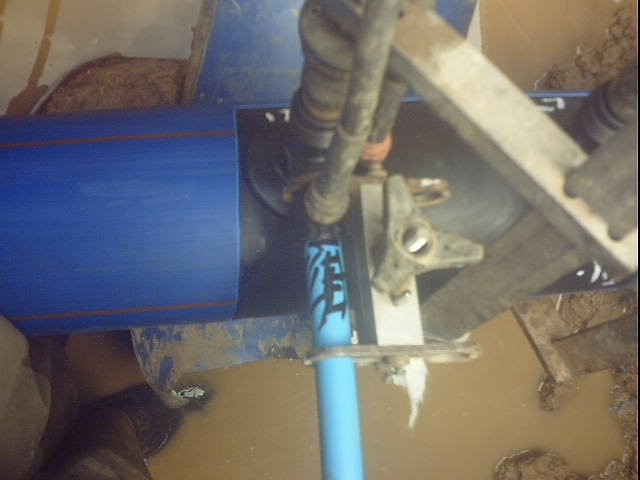
\includegraphics[width=0.3\linewidth]{images/soilcontam2.jpg}
	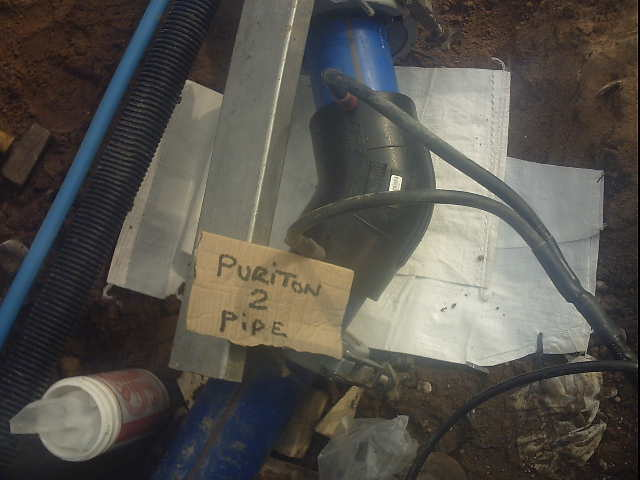
\includegraphics[width=0.3\linewidth]{images/watercontam1.jpg}
	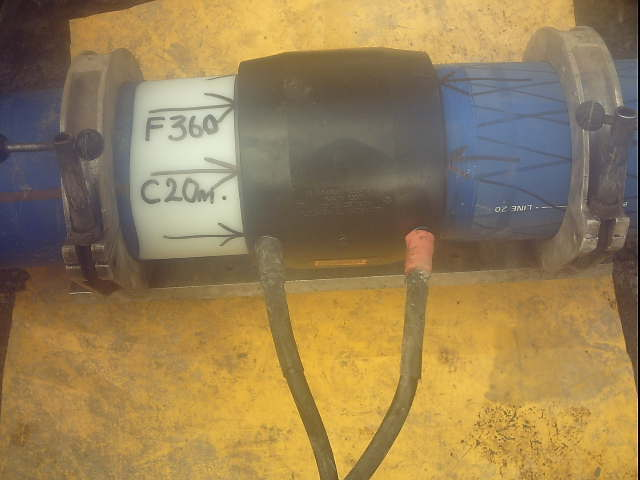
\includegraphics[width=0.3\linewidth]{images/perfect2.jpg}
	\caption{soil contamination risk (left), water contamination risk (centre), no risk (right)}
\end{figure}

These images are then manually inspected at the ControlPoint headquarters and checked for the presence of the adverse characteristics listed above. The joint is accepted and counted as finished if the number of penalty points is sufficiently low (the threshold varies from an installation contractor to the next, but 50 and above is generally considered as unacceptable). Although these characteristics are all outer observations of the pipe fitting, they have shown to be very good indicators of the quality of the weld \cite{control-point}. Manual inspection of the pipes is not only expensive, but also delaying: as images are queued for inspection, so is the completion of a pipe fitting. Contractors are often under tight operational time constraints in order to keep the shutting off of gas or water access to a minimum, so the protocol can be a significant impediment. Automated, immediate classification would therefore bring strong benefits.

\subsubsection{Formalising the problem: Multi-Instance Multi-Label Supervised Learning}

The problem of learning to classify pipe weld images from a labelled dataset is a Multi-Instance Multi-Label (MIML) supervised learning classification problem \cite{MIML}: \\

%\begin{changemargin}{1cm}{1cm}  
\indent Given an instance space $\mathcal{X}$, a set of class labels $\mathcal{Y}$, a dataset $\{(X_{1},Y_{1}),(X_{2},Y_{2}), ..., (X_{n},Y_{n})\}$,\\ 
\indent learn a function $f : 2^{\mathcal{X}} \rightarrow 2^{\mathcal{Y}}$ where\\  
\indent \indent $X_{i} \subseteq \mathcal{X}$ is a set of instances $\{x_{1}^{(i)}, x_{2}^{(i)}, ..., x_{p_{i}}^{(i)}\}$\\   
\indent \indent $Y_{	i} \subseteq \mathcal{Y}$ is the set of classes $\{y_{1}^{(i)}, y_{2}^{(i)}, ..., y_{p_{i}}^{(i)}\}$ such that $x_{j}^{(i)}$ is an instance of class $y_{j}^{(i)}$ 
\indent \indent $p_{i}$ is the number of class instances (i.e.\ labels) present in $X_{i}$.\\
%\end{changemargin}


This differs from the traditional supervised learning classification task, formally given by: \\ 

\indent Given an instance space $\mathcal{X}$, a set of class labels $\mathcal{Y}$, a dataset $\{(x_{1},y_{1}),(x_{2},y_{2}), ..., (x_{n},y_{n})\}$,\\ 
\indent learn a function $f : \mathcal{X} \rightarrow \mathcal{Y}$ where\\  
\indent \indent $x_{i} \in \mathcal{X}$ is an instance \\   
\indent \indent $y_{	i} \in \mathcal{Y}$ is the class of which $x_{i}$ is an instance.\\

In the case of MIML, not only are there multiple instances present in each case, but the number of instances is unknown. MIML has been used in the image classification literature when one wishes to identify all objects which are present in the image \cite{MIML}. Although in this case, the motivation is to look out for a specific set of pipe weld visual characteristics, the problem is actually conceptually the same; the number of identifiable classes is simply lower.

\subsubsection{Supervised Learning}

Learning in the case of classification consists in using the dataset $\mathcal{D}$ to find the hypothesis function $f^{h}$ that best approximates the unknown function $f^{*} : 2^{\mathcal{X}} \rightarrow 2^{\mathcal{Y}}$ which would perfectly classify any subset of the instance space $\mathcal{X}$. Supervised learning arises when $f^{*}(x)$ is known for every instance in the dataset, i.e.\ when the dataset is labelled and of the form $\{(x_{1},f^{*}(x_{1})),(x_{2},f^{*}(x_{2})), ..., (x_{n},f^{*}(x_{n}))\}$. This means that $|\mathcal{D}|$ points of $f^{*}$ are known, and can be used to fit $f^{h}$ to them, using an appropriate cost function $\mathcal{C}$. $\mathcal{D}$ is therefore referred to as the \textit{training set}. 

Formally, supervised learning therefore consists in finding

\begin{equation}
\label{learning: optimisation equation}
  f^{h} = \operatornamewithlimits{argmin}\limits_{\mathcal{F}}\operatorname{\mathcal{C}}(\mathcal{D})
\end{equation}
  
where $\mathcal{F}$ is the chosen target function space in which to search for $f^{h}$ . \\

\subsubsection{Approximation vs Generalisation}

It is important to note that supervised learning does not consist in merely finding the function which best fits the training set - the availability of numerous universal approximating function classes (such as the set of all finite order polynomials) would make this a relatively simple task \cite{univ-approx}. The crux of supervised learning is to find a hypothesis function which fits the training set well \textit{and} would fit well to any subset of the instance space. In other words, approximation and generalisation are the two optimisation criteria for supervised learning, and both need to be incorporated into the cost function.\\

\subsection{Architecture of a Deep Convolutional Neural Network with Rectified Linear Neurons}

A most complete and concise review of ConvNet architecture can be found in "Stochastic Pooling" paper. You could imitate the structure and expound on every single point with image examples. \\

Learning a hypothesis function $f^{h}$ comes down to searching a target function space for the function which minimises the cost function. A function space is defined by a parametrised function equation, and a parameter space. Choosing a deep convolutional neural network with rectified linear neurons sets the parametrised function equation. By explaining the architecture of such a neural network, this subsection justifies the chosen function equation. As for the parameter space, it is $\mathbb{R^{P}}$ (where P is the number of parameters in the network); its continuity must be noted as this enables the use of gradient descent as the optimisation algorithm (as is discussed later). \\



\subsubsection{Models of Neurons}

Before we consider the neural network architecture as a whole, let us start with the building block of a neural network: the neuron (mathematically referred to as the \textit{activation function}). Two types of neuron models are used in current state-of-the-art implementations of deep convolutional neural networks: the rectified linear unit and the softmax unit (note that the terms "neuron" and "unit" are used interchangeably). In order to bring out their specific characteristics, we shall first consider two other compatible neuron models: the binary threshold neuron, which is the most intuitive, and the hyperbolic tangent neuron, which is the most analytically appealing. It may also help to know what is being modelled, so a very brief look at a biological neuron shall first be given.

\paragraph{Multipolar Biological Neuron}

\begin{figure}[h!]
	\centering
	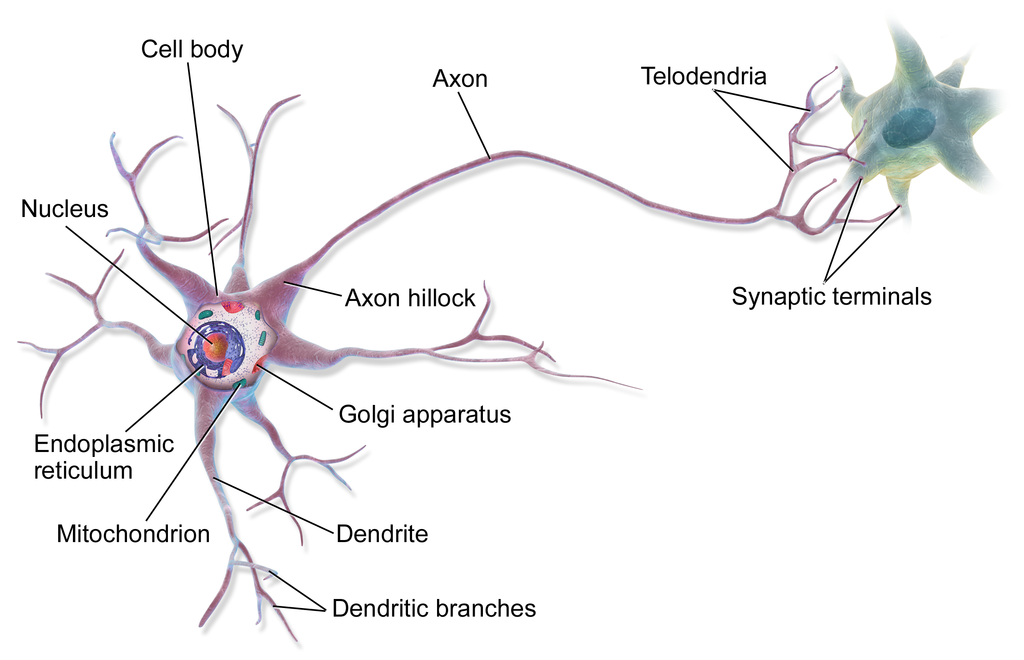
\includegraphics[scale=0.3]{images/Biological_Neuron.png}
	\caption{a multipolar biological neuron}
\end{figure}

A multipolar neuron receives electric charges from neighbouring incoming neurons through its dendritic branches, and sends electric charges to its neighbouring outgoing neurons through its axon. Neurons connect at synapses, which is where the tip of the telodendria of one neuron is in close vicinity of the dendritic branch of another neuron. Because a single axon feeds into all of the telodendria but mutiple dendritic branches feed into the axon hillock, a neuron receives multiple inputs and sends out a single output. Similarly, all of the neuron models below are functions from a multidimensional space to a unidimensional one.\\

\paragraph{Binary Threshold Neuron}
\begin{equation}
y = \begin{cases} 1 & \mbox{if } M <= b + \sum\limits_{i=1}^k x_{i}\cdot w_{i}  \text{ , where } M \text{ is a threshold parameter} \\ 
				  0 & \mbox{otherwise} \end{cases}
\end{equation} \\

Intuitively, $y$ takes a hard decision, just like biological neurons: either a charge is sent, or it isn't. $y$ can be seen as producing spikes, $x_{i}$ as the indicator value of some feature, and $w_[i]$ as a parameter of the function that indicates how important $x_{i}$ is in determining $y$. Although this model is closer than most most to reality, the function is not differentiable, which makes it impossible to use greedy local optimisation learning algorithms - such as gradient descent - which need to compute derivatives involving the activation functions.

\paragraph{Logistic Sigmoid Neuron} 
\begin{equation}
\label{sigmoid neuron}
y = \frac{1}{1 + \exp(-z)} \text{, where } z = \sum\limits_{i=1}^k x_{i}\cdot w_{i}
\end{equation}

Like the binary threshold neuron, the output domain of this neuron is bounded by 0 and 1. But this time, the function is fully differentiable. Moreover, it is nonlinear, which helps to increase performance \cite{DL-book}. To see why, the graph plot below lends itself to the following intuition: if the input x is the amount of evidence for the components of the feature that the neuron detects, and y is the evidence for the feature itself, then the marginal evidence for the feature is decreasing with the amount of evidence for its components (in absolute value terms). 

\begin{figure}[h!]
	\centering
	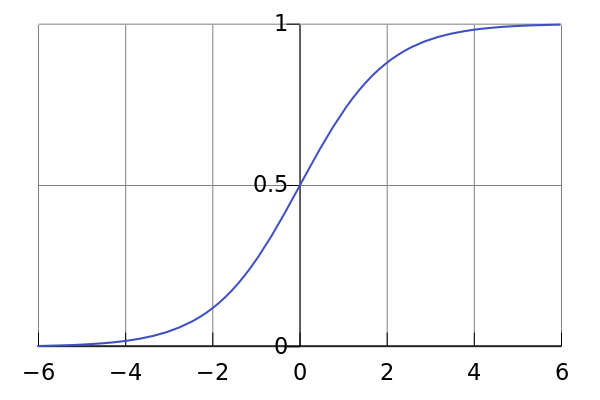
\includegraphics[scale=0.3]{images/sigmoid.png}
	\caption{single-input logistic sigmoid neuron}
\end{figure}

This is like saying that to completely convince y of the total presence or absence of the feature, a lot of evidence is required. However, if there is not much evidence for either case, then y is more lenient. 
A disadvantage of this neuron model is that it is computationally expensive to compute.
                
\paragraph{Rectified Linear Neuron}
\begin{equation}
\label{relu}
y = \max\{0, b + \sum\limits_{i=1}^k x_{i}\cdot w_{i}\}
\end{equation}

As can be seen in the graph plot below, the rectified linear neuron is neither fully differentiable (not at $0$), nor bounded above. Moreover, it only has two slopes, so its derivative with respect to $x_{i}$ can only be one of two values: $0$ or $w_{i}$. Although this may come as a strong downgrade in sophistication compared to the logistic sigmoid neuron, it is so much more efficient to compute (both its value and its partial derivatives) that it enables much larger network implementations\cite{krizhevsky}. Until now, this has more than offset the per-neuron information loss - and saturation risks - of the rectifier versus the sigmoid unit \cite{rectifier}. \\

ReLU introduces a non-linearity with its angular point (a smooth approximation to it is the softplus $f(x) = \log(1 + e^x)$). \\

Add the maths for why ReLU train faster. \\

Explain also the no neighbouring cancellations in pooling. \\

\begin{figure}[h!]
	\centering
	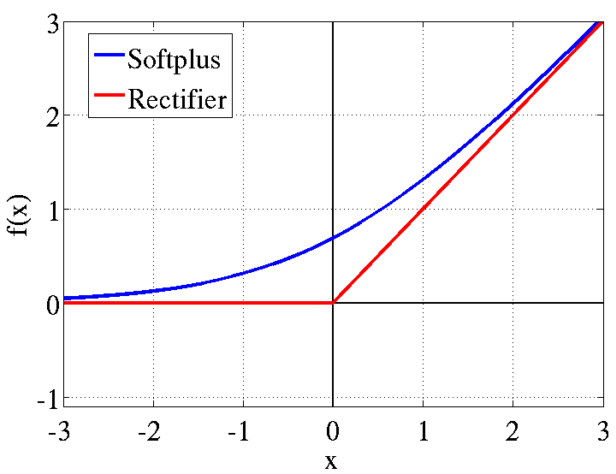
\includegraphics[scale=0.3]{images/rectifier.png}
	\caption{single-input rectified linear neuron}
\end{figure}

\paragraph{Softmax Neuron}
\begin{equation}
\label{}
y_{j} = \frac{\exp(z_{j})}{\sum\limits_{i=1}^k\exp(z_{i})} \text{, where } z_{j} = \sum\limits_{i=1}^k x_{i}\cdot w_{i,j} + b
\end{equation}

The equation of a softmax neuron needs to be understood in the context of a layer of $k$ such neurons within a neural network: therefore, the notation $y_{j}$ corresponds to the output of the $j^{th}$ softmax neuron, and $w_{i,j}$ corresponds to the weight of $x_{i}$ as in input for the $j^{th}$ softmax neuron. A layer of softmax neurons distinguishes itself from others in that neighbouring neurons interact with each other: as can be seen from the equation, the input vectors of all the softmax neurons $z_{1}, z_{2}, ..., z_{k}$ serve to enforce $\sum\limits_{i=1}^k y_{i} = 1$. In other words, the vector $(y_{1}, y_{2}, ..., y_{k})$ defines a probability mass function. This makes the softmax layer ideal for classification: neuron $j$ can be made to represent the probability that the input is an instance of class $j$. Another attractive aspect of the softmax neuron is that its derivative is quick to compute: it is given by $\frac{dy}{dz} = \frac{y}{1-y}$. \\

intuition: Bishop textbook: "softmax function, as it represents
a smoothed version of the ‘max’ function because, if ak ? aj for all j ?= k, then p(Ck|x) ? 1, and p(Cj|x) ? 0."


\subsubsection{Feed-Forward Architecture}

A feed-forward neural network is a representation of a function in the form of a directed acyclic graph, so this graph can be interpreted both biologically and mathematically. A node represents a neuron as well as an activation function $f$, an edge represents a synapse as well as the composition of two activation functions $f \circ g$, and an edge weight represents the strength of the connection between two neurons as well as a parameter of $f$. The figure below (taken from \cite{DL-book}) illustrates this.

\begin{figure}[h!]
	\centering
	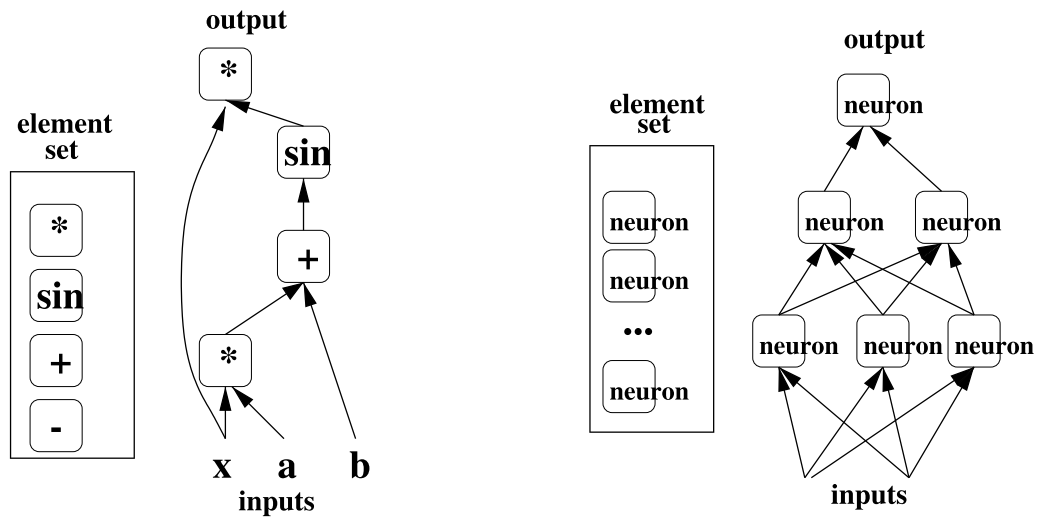
\includegraphics[scale=0.3]{images/NN_math_rep.png}
	\caption{graphical representation of $y = x*sin(a*x+b)$ and of a feed-forward neural network}
\end{figure}

The architecture is feed-forward in the sense that data travels in one direction, from one layer to the other. This defines an input layer (at the bottom) and an output layer (at the top) and enables the representation of a mathematical function.\\

\paragraph{Shallow Feed-Forward Neural Networks: the Perceptron}

A feed-forward neural net is called a perceptron if there exist no layers between the input and output layers. The first neural networks, introduced in the 1960s \cite{DL-book}, were of this kind. This architecture severely reduces the function space: for example, with $g_{1}: x \rightarrow sin(s)$, $g_{2}: x,y \rightarrow x*y$, $g_{3}: x,y \rightarrow x+y$ as activation functions (i.e.\ neurons), it cannot represent $f(x) \rightarrow x*sin(a*x+b)$ mentioned above \cite{DL-book}. This was generalised and proved in \textit{Perceptrons: an Introduction to Computation Geometry} by Minsky and Papert (1969) and lead to a move away from artificial neural networks for machine learning by the academic community throughout the 1970s: the so-called "AI Winter" \cite{Russel & Norvig}.

\paragraph{Deep Feed-Forward Neural Networks: the Multilayer Perceptron}

The official name for a deep neural network is Multilayer Perceptron (MLP), and can be represented by a directed acyclic graph made up of more than two layers (i.e.\ not just an input and an output layer). These other layers are called hidden layers, because the "roles" of the neurons within them are not set from the start, but learned throughout training. When training is successful, each neuron becomes a feature detector. At this point, it is important to note that feature learning is what sets machine learning with MLPs apart from most other machine learning techniques, in which features are specified by the programmer \cite{DL-book}. It is therefore a strong candidate for classification tasks where features are too numerous, complex or abstract to be hand-coded - which is arguably the case with pipe weld images.\\ 

Intuitively, having a hidden layer feed into another hidden layer above enables the learning of complex, abstract features, as a higher hidden layer can learn features which combine, build upon and complexify the features detected in the layer below. The neurons of the output layer can be viewed as using information about features in the input to determine the output value. In the case of classification, where each output neuron corresponds to the probability of membership of a specific class, the neuron can be seen as using information about the most abstract features (i.e.\ those closest to defining the entire object) to determine the probability of a certain class membership. \\

To make the case for deep architectures, consider a model with the same number of parameters but fewer layers (i.e.\ a greater number of neurons per layer). Goodfellow's paper on google street view number recognition (https://www.youtube.com/watch?v=vGPI_JvLoN0&list=PLhiWXaTdsWB-3O19E0PSR0r9OseIylUM8&index=18) ran experiments to compare and found that depth is better: intuitively, if neurons are side by side, they cannot use the computation of their neighbour, whereas with depth, the neurons above can make use of the work done by the neurons below. \\	

Mathematically, it was proved in 1989 that MLPs are universal approximators \cite{MLP-univ-approx}; hidden layers therefore increase the size of the function space, and solve the initial limitation faced by perceptrons.\\


\paragraph{Deep Convolutional Neural Networks: for translation invariance}

A convolutional neural network uses a specific network topology that is inspired by the biological visual cortex and tailored for computer vision tasks, because it achieves translation invariance of the features. Consider the following image of a geranium: a good feature to classify this image would be the blue flower. This feature appears all across the image; therefore, if the network can learn it, it should then sweep the entire image to look for it. A convolutional layer implements this: it is divided into groups of neurons (called \textit{kernels}), where all of the neurons in a kernel are set to the same parameter values, but are 'wired' to different pixel windows across the image. As a result, one feature can be detected anywhere on the image, and the information of where on the image this feature was detected is contained in the output of the kernel. Below is a representation of LeNet5, a deep convolutional neural network used to classify handwritten characters. \\

(Hey, you should explain what is meant by convolution with http://colah.github.io/posts/2014-07-Understanding-Convolutions/ by using some of the images.) \\

\begin{figure}[h!]
	\centering
	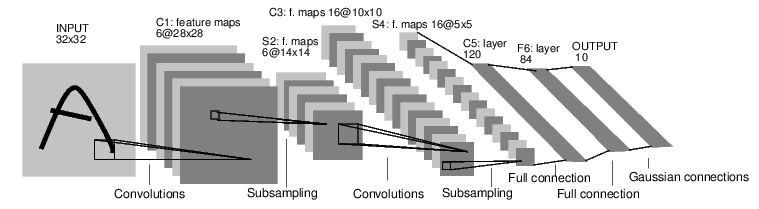
\includegraphics[scale=0.6]{images/lenet5.png}
	\caption{LeNet7 architecture: each square is a kernel}
\end{figure}

\subparagraph{Kernels}

awesome explanation of sliding kernels:
http://colah.github.io/posts/2014-07-Understanding-Convolutions/
http://docs.gimp.org/en/plug-in-convmatrix.html

example 1: dark left light right edge detector
example 2: overall edge detector
comment on how 2 is more generic, but 1 carries more precise information.
example 3: blurring
example 4: sharpening

Further, while convolution naively appears to be an O(n2) operation, using some rather deep mathematical insights, it is possible to create a O(nlog(n)) implementation. (yes, you can parallelise the convolution quite easily, each window of a kernel can be computed in parallel)

\subsubsection{Topology of Deep Neural Networks}

Now that architecture is clear, let's take a step back and consider the topology of deep neural networks. One may wonder whether it is useful to going into such abstract maths for an applied project such as this one; but doing this will provide an answer to a frequent critique of deep neural networks: "we don't know what they are doing". By proving that a deep neural network is a homeomorphism, we can provide the answer that training a deep neural network is akin to searching for a combination of projections, stretches and squashes of the input space to end up with a linearly separable configuration.

http://colah.github.io/posts/2014-03-NN-Manifolds-Topology/


\paragraph{Topology of $tanh$ Layer}

First start with mathematical definitions. \\

\subparagraph{Homeomorphism}
A function $f: X → Y$ between two topological spaces (X, TX) and (Y, TY) is called a homeomorphism if it has the following properties: 
f is a bijection (one-to-one and onto),
f is continuous,
the inverse function $f^{−1}$ is continuous (f is an open mapping). \\

Theorem: a tanh layer is a homeomorphism if the weight matrix is invertible.

$tanh$ is a continuous bijection between its input and output domains, \mathcalbb{R} and ]-1;1[, and ??? is its continuous inverse.
 A translation is also bi-continuous. However, a linear transformation is only bi-coso a $tanh$ layer is a homeomorphism. The implications of this are intuitively interesting: it means that the layer performs a continuous transformation ... \\

Since each layer is a homeomorphism, then the entire network is a homeomorphism too (

Why would we desire 

\paragraph{Topology of ReLU Layer}

Wait a second, what makes you think that the weight matrix will ever be invertible in practice? Only square matrices can be invertible, and in practice it's rare for two adjacent layers to have the same number of neurons. \\

ReLU is not a bijection between its input and output domains, \mathcalbb{R} and [0;\infty[. So a layer of ReLUs is not a homeomorphism. Does this mean we cannot study the topology of such deep neural networks? What does it imply for the type of transformations that can be applied to the data? Could you provide an animation of collapsing on an axis? \\

\paragraph{Ambient Isotopy}

definition:
http://www.cs.ucdavis.edu/~amenta/pubs/tcs-iso-qed.pdf \\

Embedding, untangling the manifold. \\

\paragraph{The Manifold Hypothesis}

Why is it important to know that we are using homeomorphisms? Because a homeomorphism guarantees the existence of an inverse continuous function. If we see the class of cat images as a manifold (cf deep spars rectifier network for phrase used to decribe this) that has been heavily tangled by being represented in the pixel space, then it's good to know that there exists a continuous function that will untangle it, since that's what the deep neural network is looking for.

Conclusion is that learning a classification task with a deep neural network is like learning how to disentangle manifolds. 


\subsubsection{Krizhevsky 2012 explained}

CAREFUL! these are notes taken from the tutorial\cite{nips-tut}. The structure is totally plagiarised. Instead, you insert pieces of content below in areas above.
video, currently on 10:20

To situate the CNN in terms of other ANNs, it may help to view a number of them in terms of depth and learning strategy:

\begin{figure}[h!]
	\centering
	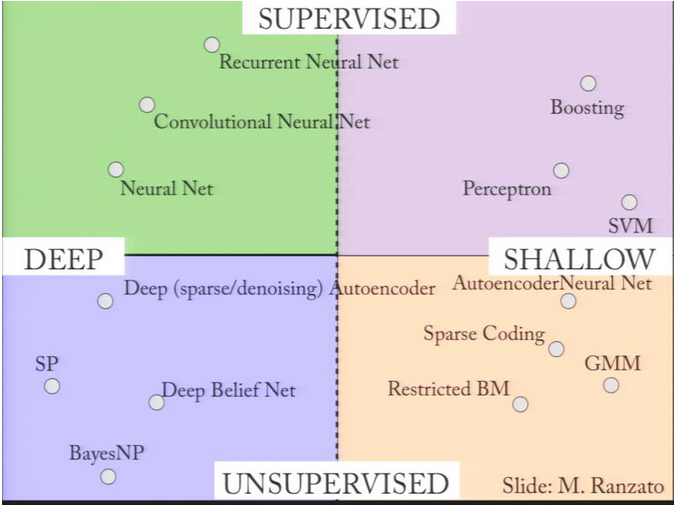
\includegraphics[scale=0.6]{images/all_neural_networks.png}
	\caption{Different kinds of ANNs}
\end{figure}


\paragraph{Operations in each layer}

images to paste: http://media.nips.cc/Conferences/2013/Video/Tutorial1A.pdf 

A convolution layer has a pixel feature i.e. filter which is convolved over the entire image, followed by a non-linearity, followed by a spatial feature, optionally followed by a normalisation between feature responses. This may seem like it comes out of nowhere, but when we look at hand-crafted successes in computer vision, the structures are similar. \\

For example consider SIFT (Scale-invariant feature transform) descriptors: they are a range of filters for edges at different angles. \\

\subparagraph{Filter aka Pixel Feature}

 
\subparagraph{Non-linearity}

\subparagraph{Pooling aka Spatial Feature}

\subparagraph{Possible Normalisation}



\paragraph{Architecture}

\paragraph{Training}

\paragraph{Results}

\subsection{Training: Backpropagation}

Now that the architecture of a deep CNN has been explained, the question remains of how to train it. Mathematically: now that the function space has been explained, the question remains of how this space is searched. In the case of feed-forward neural networks and supervised learning, this is done with gradient descent, a local (therefore greedy) optimisation algorithm. Gradient descent relies on the partial derivatives of the error (a.k.a\ cost) function with respect to each parameter of the network; the backpropagation algorithm is an implementation of gradient descent which efficiently computes these values.
  
\subsubsection{Compute Error-Weight Partial Derivatives}

Let $t$ be the target output (with classification, this is the label) and let $y = (y_{1}, y_{2}, ..., y_{P})$ be actual value of the output layer on a training case. (Note that classification is assumed here: there are multiple output neurons, one for each class).

The error is given by 
\begin{equation}
E = \mathcal{C}(t-y)
\end{equation}

where $\mathcal{C}$ is the chosen cost function. The error-weight partial derivatives are given by

\begin{equation}
\frac{\partial{E}}{\partial{w_{ij}}} = \frac{\partial{E}}{\partial{y_{i}}} \cdot \frac{\partial{y_{i}}}{\partial{net}} \cdot \frac{\partial{net}}{\partial{w_{ij}}}
\end{equation}

Since in general, a derivative $\frac{\partial{f}}{\partial{x}}$ is numerically obtained by perturbing $x$ and taking the change in $f(x)$, the advantage with this formula is that instead of individually perturbing each weight $w_{ij}$, only the unit outputs $y_{i}$ are perturbed. In a neural network with $k$ fully connected layers and $n$ units per layer, this amounts to $\Theta(k \cdot n)$ unit perturbations instead of $\Theta(k \cdot n^{2})$ weight perturbations (note that the bound on weight perturbations is no longer tight if we drop the assumption of fully connected layers). \\

The error being shown is the negative of the log probability of the likelihood function:
\begin{equation}
-\frac{1}{n}\sum\limits_{i=1}^n ln(f(W|x_i))
\end{equation}
Where f is the learned function. This is the cross entropy, but it also elegantly evaluates to MLE. In other words, we are choosing the parameters of the model to maximise the likelihood of the data (to make the observed events i.e.\ the training set as highly probable as possible). Do the proof with joint probability of independent events etc. \\


\subsubsection{Update Weight Values (with Gradient Descent)}

The learning rule is given by $w_{i,t+1} = w_{i,t+1} + \tau \cdot \frac{\partial{E}}{\partial{w_{i,t}}}$

Visually, this means that weight values move in the direction the will reduce the error quickest, i.e.\ the direction of steepest descent on the error surface is taken. Notice that given the learning rule, gradient descent converges (i.e.\ $w_{i,t+1}$ equals $w_{i,t+1}$) when the partial derivative reaches zero. This corresponds to a local minimum on the error surface. In the figure below, two potential training sessions are illustrated. The minima attained in each cases are not the same. This illustrates a strong shortcoming with backpropagation: parameter values can get stuck in poor local minima.

\begin{figure}[h!]
	\centering
	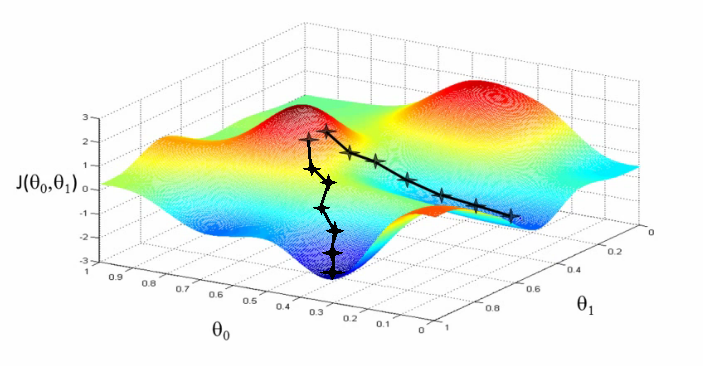
\includegraphics[scale=0.8]{images/local_minima.png}
	\caption{an error surface with poor local minima}
\end{figure}


% \paragraph{cost functions}
% MSE, cross-entropy for softmax

\paragraph{Training, Validation and Test Sets}

As mentioned previously, learning is not a mere approximation problem because the hypothesis function must generalise well to any subset of the instance space. Approximation and generalisation are incorporated into the training of deep neural networks (as well as other models \cite{train&test}) by separating the labelled dataset into a training set, a validation set and a test set. The partial derivatives are computed from the error over the training set, but the function that is learned is the one that minimises the error over the validation set, and its performance is measured on the test set. The distinction between training and validation sets is what prevents the function from overfitting the training data: if the function begins to overfit, the error on the validation set will increase and training will be stopped. The distinction between the test set and the validation set is to obtain a stochastically impartial measure of performance: since the function is chosen to minimise the error over the validation set, there could be some non-negligible overfit to the validation set which can only be reflected by assessing the function's performance on yet another set.

% \paragraph{Dropout}


\subsection{Challenges specific to the Pipe Weld Classification Task}

A number of significant challenges have arisen from this task: multi-tagging, domain change, small dataset size (by deep learning standards) and class imbalance. Before going into them, an overview of the data is given below. \\

\subsubsection{Data Overview}
% \subsubsection{Visual Inspection}
% \subsubsection{Analysis}
% \paragraph{ANOVA}
% \paragraph{t-SNE}


ControlPoint recently upgraded the photographical equipment with which photos are taken (from 'Redbox' equipment to 'Bluebox' equipment), which means that the resolution and finishing of the photos has been altered. There are 113,865 640x480 'RedBox' images. There are 13,790 1280x960 'BlueBox' images. Label frequencies for the Redbox images are given below.

\begin{table}[h]
   \centering
    \begin{tabular}{|l|c|c|}
    \hline
    Characteristic                              & ~ Redbox Count  & ~ Bluebox Count \\ \hline
    Fitting Proximity                           & ~  1,233        & ~ 32      \\
    Inadequate Or Incorrect Clamping            & ~ 1,401         & ~ 83      \\
    Joint Misaligned                            & ~ 391           & ~ 35      \\
    No Clamp Used                               & ~ 8,041         & ~ 1,571   \\
    No Ground Sheet                             & ~  30,015       & ~ 5,541   \\
    No Insertion Depth Markings                 & ~ 17,667        & ~ 897     \\
    No Visible Evidence Of Scraping Or Peeling  & ~ 25,499        & ~ 1,410   \\
    No Visible Hatch Markings                   & ~ 28,155        & ~ 3,793   \\
    Other                                       & ~  251          & ~ 103     \\
    Photo Does Not Show Enough Of Clamps        & ~ 5,059         & ~ 363     \\
    Photo Does Not Show Enough Of Scrape Zones  & ~ 21,272        & ~ 2,545   \\
    Soil Contamination High Risk                & ~ 6,541         & ~ 3       \\
    Soil Contamination Low Risk                 & ~ 10            & ~ N/A     \\
    Soil Contamination Risk                     & ~ ?             & ~ 529     \\
    Unsuitable Photo                            & ~ 2             & ~ N/A     \\
    Unsuitable Scraping Or Peeling              & ~ 2,125         & ~ 292     \\
    Water Contamination High Risk               & ~ 1,927         & ~ 9       \\
    Water Contamination Low Risk                & ~ 3             & ~ 7       \\
	Water Contamination Risk                    & ~ ?             & ~ 296     \\
     \hline
    Perfect (no labels)                         & ~ 49,039        & ~ 4,182   \\
    \hline
    \end{tabular}
    \caption {Count of Redbox images with given label}
\end{table} 

\subsubsection{Multi-Tagging}:

As mentioned earlier, training images contain varying numbers of class instances; this uncertainty complexifies the training task.

\subsubsection{Domain Change}:

Domain change can be lethal to machine vision algorithms: for example, a feature learned (at the pixel level) from the 640x480 Redbox images could end up being out of scale for the 1280x960 Bluebox images. However, this simple example is not relevant to a CNN implementation, since the largest networks can only manage 256x256 images, so Bluebox and Redbox images will both be downsized to identical resolutions. However, more worrying is the difference in image sharpness between Redbox and Bluebox images, as can be seen below. It remains to be seen how a CNN could be made to deal with this type of domain change.

\begin{figure}[h!]
	\centering
	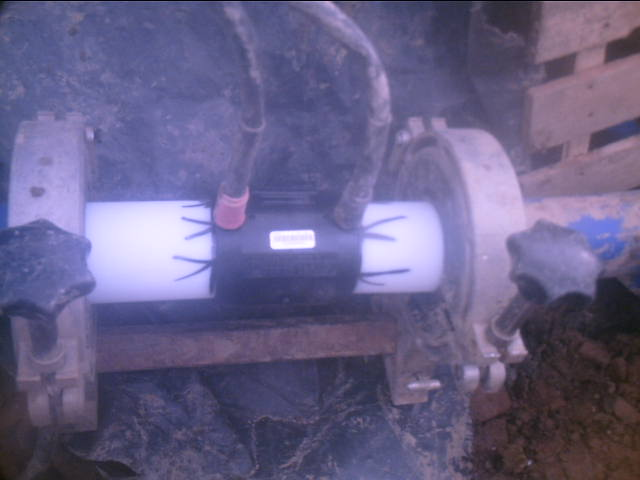
\includegraphics[scale=0.34]{images/perfect3.jpg}
	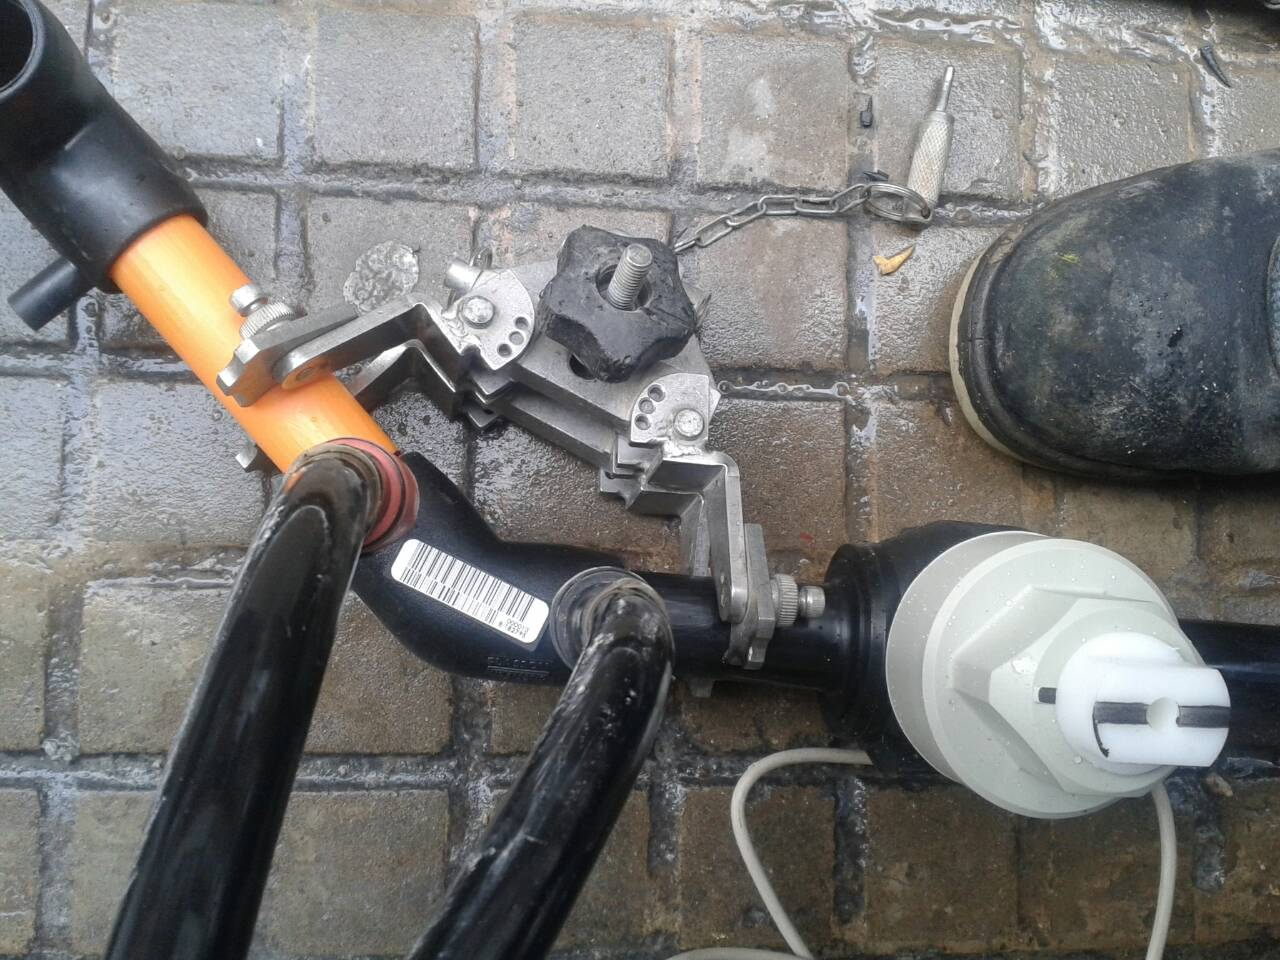
\includegraphics[scale=0.17]{images/niceBluebox_100974.jpg}
	\caption{left: a Redbox photo - right: a Bluebox photo}
\end{figure}

Nevertheless, evidence has been found to suggest that deep neural networks are robust to it: an experiment run by Donahue et al on the \textit{Office} dataset \cite{office}, consisting of images of the same products taken with three different types of photographical equipment (professional studio equipment, digital SLR, webcam) found that their implementation of a deep convolutional neural network produced similar feature representations of two images of the same object even when the two images were taken with different equipment, but that this was not the case when using SURF, the currently best performing set of hand-coded features on the \textit{Office} dataset \cite{surf}. \\

\subsubsection{Small Dataset Size}

Alex Krizhevsky's record-breaking CNN was trained on 1 million images \cite{krizhevsky}. Such a large dataset enabled the training of a 60-million parameter neural network, without leading to overfit. In this case, there are 'only' 127,000, and 43\% of them are images of "perfect" welds, meaning that these are label-less. Training a similarly sized network leads to overfit, but training a smaller network could prevent the network from learning sufficiently abstract and complex features for the task at hand. A solution to consider is that of transfer learning \cite{transfer-learning}, which consists in importing a net which has been pretrained in a similar task with vast amounts of data, and to use it as a feature extractor. This would bring the major advantage that a large network architecture can be used, but the number of free parameters can be reduced to fit the size of the training set by "freezing" backpropagation on the lower layers of the network. Intuitively, it would make sense to freeze the lower (convolutional) layers and to re-train the higher ones, since low-level features (such as edges and corners) are likely to be similar across any object recognition task, but the way in which these features are combined are specific to the objects to detect.

\subsubsection{Class Imbalance}

The dataset suffers from a similar adverse characteristic to that of medical datasets: pathology observations are significantly less frequent that healthy observations. This can make mini-batch training of the network especially difficult. Consider the simple case of training a neural network to learn the following labels: No Clamp Used, Photo Does Not Show Enough Of Clamps, Clamp Detected (this label is not in the list, but can be constructed as the default label). Only 8\% of the Redbox images contain the first label, and only 5\% contain the second label, so if the partial derivatives of the error are computed over a batch of 128 images (as is the case with the best implementations \cite{krizhevsky},\cite{transfer-learning}, \cite{decaf}), one can only expect a handful of them to contain either of the first two labels. Intuively, one may ask: how could I learn to recognise something if I'm hardly ever shown it?\\

One possible solution would be to use a different cost function: the F-measure \cite{f-measure}, which is known to deal with these circumstances. Although the F-measure has been adapted to into a fully differentiable cost function (which is mandatory for gradient descent), there currently exists no generalisation of it for the case of $n \ge 2$
classes. Moreover, one would need to ensure that the range of the error is as large as possible for a softmax activation unit, whose own output range is merely $[0;1]$. \\ \\




\clearpage

\section{Analysis 1: ReLU Activation}

Talk about the mathematical intuition.

\section{Analysis 2: Early Stopping}

Combine your intuition with the stuff from that conference, about gradient descent and extra polynomial order.

\section{Task 1: Generic Clamp Detection}

Justify multiple binary classifiers in light of Chao Wu's multi-label classification work: http://www.aicit.org/aiss/global/paper_detail.html?jname=AISS&q=1061


\subsection{Motivations}

Clamp detection was suggested by ControlPoint as a simple test run for training a CNN on their dataset. It was a standard single-tag task with few classes, so implementation was not as difficult as multi-tag, and the detection task in itself was deemed simple since clamps are large objects which would be easy to see. Moreover, four significant obstacles arose: non-converging error rates, class imbalance, data complexity, and mis-labelling.\\

\subsection{Design}

\subsubsection{AlexNet: State-of-the-art Benchmark}

Winner of ILSVRC 2012 by far. Decent out-of-the-box benchmark for rapid evaluation of data complexity. \\
Trained on a bigger dataset, so expected overfit to occur quickly. \\

\subsubsection{Network Architecture: Large-Scale Convolutional Neural Network}

find the image for AlexNet with the maps and kernels and stuff.

\paragraph{Convolutional Layer}

\subparagraph{Convolution}

\subparagraph{Pooling}

Why do conv layers 3 and 4 not have it? \\

\subparagraph{Normalisation}

Why do conv layers 3 and 4 not have it? \\

\paragraph{Fully Connected Layer}

\paragraph{Softmax Output Layer}


\subsection{Implementation}

\subsubsection{Cuda-Convnet: An Out-of-the-box API}

Cuda-Convnet is a GPU implementation of a deep convolutional neural network implemented in CUDA/C++. It was written by Alex Krizhevsky to train the net that set ground-breaking records at the ILSVRC 2012 competition, and subsequently open-sourced. However, parts of his work are missing and his open source repository is not sufficient to reproduce his network. In order to do so, data batching scripts were written for turning raw .jpg images and separate .dat files into pickled python objects each containing 128 stacked jpg values in matrix format with RGB values split across, and a dictionary of labels and metadata for the network. \\

Wrote scripts to pre-process the data because Cuda-Convnet and noccn don't provide everything. Had to write scripts to:
\begin{itemize}
\item get all labels
\item visually inspect random samples of the data
\item leave out images tagged as poor
\item write the data in the xml format that cuda-convnet's batching API can read
\item potentially treat unlabelled images as an extra class
\item potentially leave out classes 
\item potentially merge classes
\item randomly remove images to reach given class balance ratio
\item unit tests for all of the above
\end{itemize}
The scripts are written in python and the code is ~800 lines.


\subsubsection{Hardware: NVidia GeForce GTX 780}

CUDA-enabled GPU. How many teraflops? Which operations are parallelised? 
First a GeForce GTX 780 with 4GB RAM. 

\subsubsection{Summary: Considerable Unforeseen Challenges}

DOES THIS SUBSUBSECTION REALLY BELONG HERE? yes I would say so, but may need to be edited so that it just mentions how tough the task turned out to be, and that the obstacles which were discovered lead to devising a new task, that of joint-type classification. Perhaps also mention that unsupervised learning was considered to deal with the mis-labelled data, the reasons for why this was put aside (discussions with ControlPoint), but that it would make for interesting further research? Maybe it should be renamed to summary, and be included as final subsubsection of every implementation subsection? \\

Several weeks into training, it was discovered that in the case of tapping-T joints, for the Redbox images, the glint of a slim portion of a clamp is sufficient to judge it present. \\

\begin{figure}[h!]
	\centering
	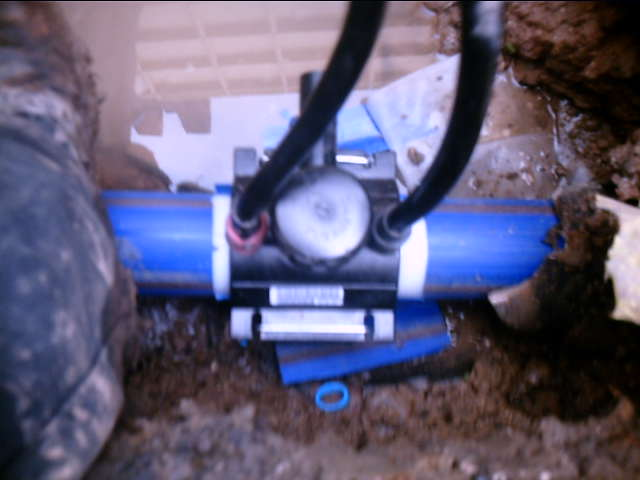
\includegraphics[width=0.35\linewidth]{images/tapping-T.jpg}
	\caption{The clamp wraps around under the pipe - the glint of a metal rod gives it away}
\end{figure}

Worse still, sometimes the presence of clamps "doesn't count": these are cases for which the purpose of the clamp is other than to secure the welding. Therefore, if such a clamp is present, but the clamp that serves to secure the weld is absent, then the image is assigned the "No Clamps" label. For example, bottom left, a clamp can clearly be seen, but it's not a weld clamp. So this image should have a "No Clamps" flag raised (sadly, it doesn't). Bottom right: the thin metallic clamp that is fastened on the vertical pipe is not the clamp we're interested in. The glint from the thin metallic rod going along the thick, horizontal pipe tells us that a tapping-T clamp is present, even though that clamp is hidden underneath the pipe. 

\begin{figure}[h!]
	\centering
	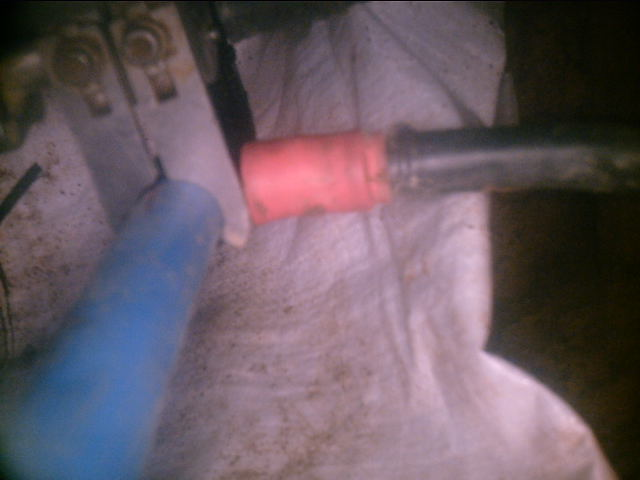
\includegraphics[width=0.35\linewidth]{images/truly_confusing_1.jpg}
	\caption{This clamp is not a weld clamp}
	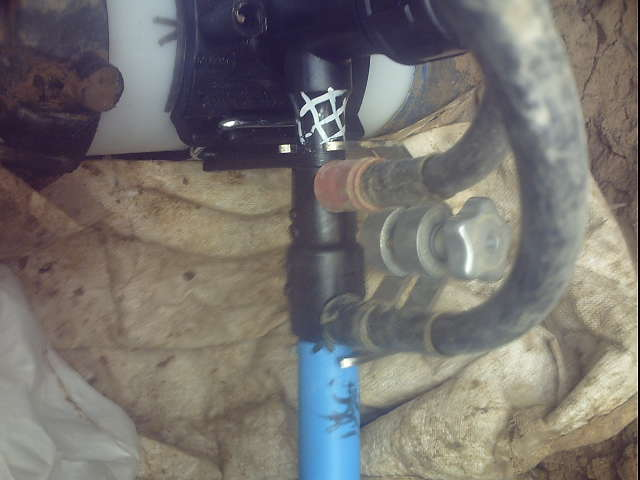
\includegraphics[width=0.35\linewidth]{images/truly_confusing_2.jpg}
	\caption{The clamp on the vertical rod is not a weld clamp}
\end{figure}

This makes learning very difficult, as a class can be pictured as a disjoint set of subclasses, some of which fine-grained, and that one subclass could trigger a false positive of another class.\\

The solution was to train a classifier capable of recognising the type of joint having been welded, using the small subset of data which contained joint-type labels, in order to try and tag the remaining dataset. The advantage of knowing the joint-type is that we can isolate clamp types, and train a classifier on s single type of clamp. That way, the learning task is simplified, and one is able to focus on the other challenges. \\


\subsection{Experimentation}

\subsubsection{Non-Converging Error Rates}

The training produced confusing results. LOOK THROUGH ENTIRE DOCUMENT, when talking about this training, the classification validation error achieved was 11\%, not 40\%! It may also be good to get a test error.

They were trained on the clamp detection task using the Redbox data only. The purpose of these models is to set a benchmark for the difficulty of the classification task, by taking several out-of-the-box network configurations: namely, those found on open source projects or detailed in papers \cite{krizhevsky},\cite{transfer-learning}, \cite{decaf}. \\

The classification task is a challenging one: indeed, none of the training sessions have shown any signs of parameter convergence, as the below plot of the training and validation errors over batch iterations can show. These results are very confusing: backpropagation is guaranteed to converge [cite! go into more detail about this! include the proof in your background!], and yet both training and validation errors seem stuck in volatile periodicity.

You should also justify why you are not bothering with the test error! Because test error optimum is obtained at validation error optimum; test error is merely a truly impartial measure of performance. A bunch of research contents itself with validation error when merely iterating through various models. 

\begin{figure}[h!]
	\centering
	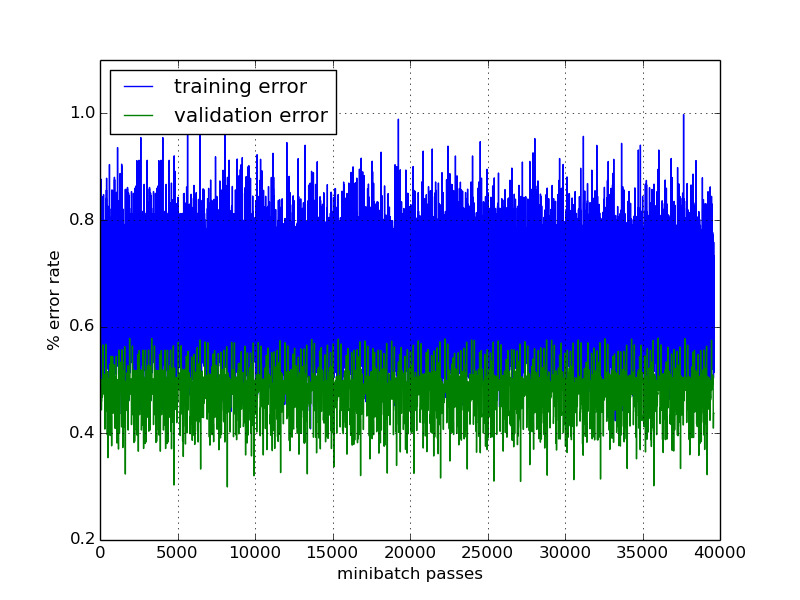
\includegraphics[scale=0.5]{images/test_run.png}
	\caption{Test Run Training Results}
\end{figure}

The error being shown is the negative of the log probability of the likelihood function:
\begin{equation}
-\frac{1}{n}\sum\limits_{i=1}^n ln(f(W|x_i))
\end{equation}
Where f is the cost function I think. So in this case it is the cross entropy I think. (Verify this, provide intuition).\\

A number of potential explanations for the volatile periodic error rates were considered:
\begin{itemize}
\item The learning rates are too high (the minimum gets 'overshot' even when the direction of partial derivatives is correct)
\item The dropout rate is too high (dropout is a technique which consists in randomly dropping out neurons from the net at every iteration to prevent overfit - but it also means that a different model is tested every time)
\item The number of parameters is too high (the out-of-the-box implementation contains millions of parameters, which is more than than the number of training cases, so collinearities between the parameters cannot even be broken, and most of them are rendered useless)
\item Class imbalance (not enough information about the clampless classes to be able to learn feature for them)
\item Mis-labeled data (at the time of human tagging of these images, tags were left out) \ldots
\item The error rates are not computed correctly \ldots
\end{itemize}


\paragraph{Increase Test Error Precision}

By computing the test error on a large and unchanging sample of images, one obtains more precise estimates, and convergence can clearly be seen.

\begin{figure}[h!]
	\centering
	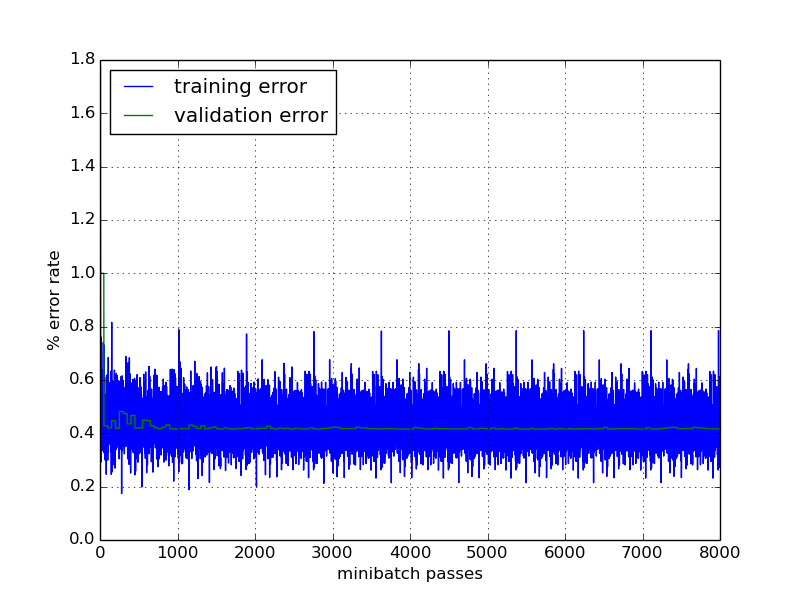
\includegraphics[scale=0.5]{images/increase_test_precision.png}
	\caption{test and validation error rates for clamp detection after fixing a large test range}
\end{figure}

I trained AlexNet on 100k images of 3 different classes with class imbalance (1 class takes up 90\% of data), ~40\% mis-labelling, and a very small learning rate (0.0001). The emerging periodicity of the training error corresponds to the number of batches, so it looks like the parameters have stopped changing, ie the network has reached a local minimum (flesh out the intuition for why periodicity implies convergence, just going around in the same circle). Why does no overfitting take place? There is not much data compared to capacity of the network, there is a weight decay of 0.0005,  there is no dropout. Since overfitting hasn't been reached, maybe this is a poor local minimum?\\

Francis Quintal Lauzon: I would tend to think learning was indeed stuck, though I would not go so far as to suggest this is caused by a local minimum.
Indeed, I have sometimes seen long plateaus followed by sudden steep drop in error.  One way I see this is learning with a given learning rate and reducing the learning rate when validation error (or rather, a smoothed version of the validation error) stops going down.  This suggest than rather being stuck at a local minima, learning is simply blundering around some minimum, may be because of a combination of the local shape of the cost surface and learning steps too large. \\

Plateau hypothesis: on the image I show only 10 epochs, but I trained it for 44 epochs and the periodicity extends all the way. When you were experiencing plateaus, did they stretch over more than 1 epoch? because to me, this periodicity suggests roughly the same gradients are repetitively being computed at the same locations on the error surface, so no good keeping on going. 

Learning rate hypothesis: so you are suggesting that the minimum keeps getting overshot. But 0.0001 learning rate is already very small no?

I guess another possibility is that I'm zigzagging in a very tight bowl, but seems unlikely it would go on for as long as 40 epochs?\\

Francis Quintal Lauzon: I trained on much larger (though highly correlated) dataset so I never trained for 44 epochs.  I did use learning rate of the same magnitude you are using and still, reducing it after a plateau does help (in my experience).  If you are using momentum, you also might want to reset any momentum to zero after facing a plateau (this might helps as well).\\


Another striking aspect is how volatile the training error is, even when the test error is stable. That the training error is computed correctly was checked by training an out-of-the-box net on a well-documented task: MNIST. Therefore, it was established that in this setup, the training error is indeed volatile and periodic despite the validation error converging, and that an explanation must exist. This could be interpreted as the network's parameters having converged to values that make it good on certain batches, and bad on others. What is curious is that this would suggest that the contents of some batches are very different from one another (unless one considers the paper "Intriguing Properties of Neural Networks"). Therefore, it might be interesting to look at these batches in detail. \\

\paragraph{Alter Momentum}

What is momentum for?

the intuition (maybe wrong): if a smaller learning rate and zero momentum could help you deal with a plateau, it means that moving in very small steps is better. but if a plateau is a continuous flat surface, then surely a smaller step will take you longer to reach the other side? 
on the other hand, if you're in a very tight and stretched bowl, or if there's a very narrow ditch surrounded by a plateau, then the smaller step will help?

\subparagraph{Increase}

Is that used to get past the local minimum? Or is it used to rush past a plateau?

\begin{figure}[h!]
	\centering
	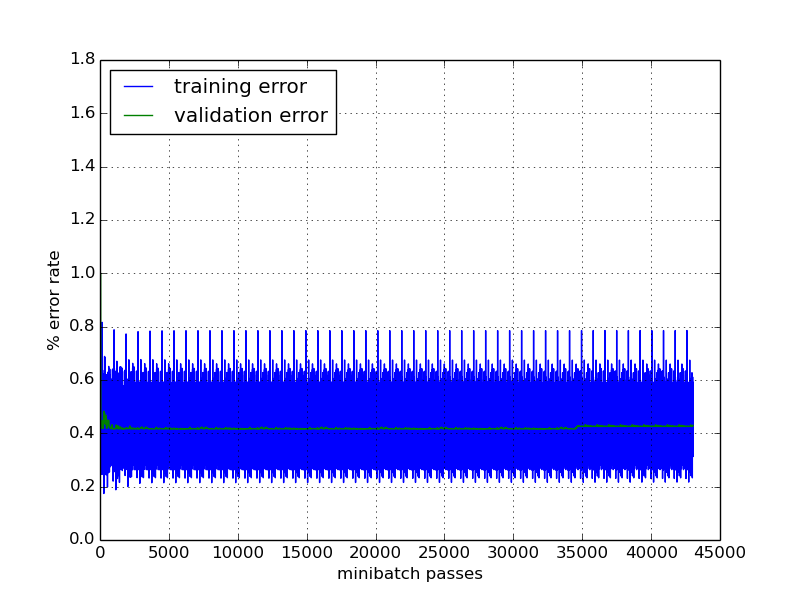
\includegraphics[scale=0.5]{images/raise_momentum.png}
	\caption{test and validation error rates for clamp detection after raising momentum}
\end{figure}

Barely noticeable change in train error: still periodic, slightly different shape of period. Slight increase in test error though. Can interpret that weight updates are slightly less optimal since they don't follow the direction given by the gradients, since there's this extra momentum factor, which is bigger.

\subparagraph{Decrease}

Because Francis Quintal Lauzon says so. But does he mean to reduce it once you're done with the plateau?

\begin{figure}[h!]
	\centering
	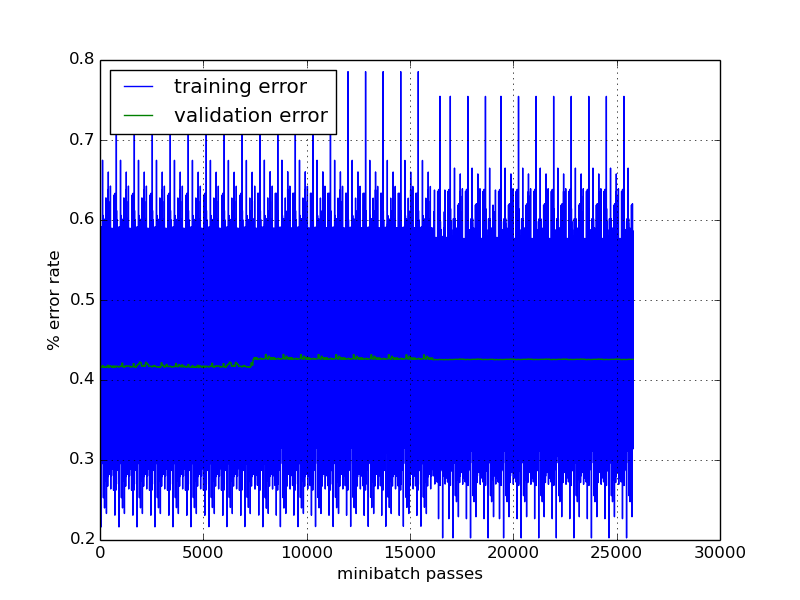
\includegraphics[scale=0.5]{images/change_momentum.png}
	\caption{test and validation error rates for clamp detection after setting momentum to zero}
\end{figure}

The training error decreases a little on average (would be good to assert this statistically). Once again, because momentum is not 	distorting direction of descent.

The test error stops to jitter completely. So the tiny pulses observed during convergence (i.e. between 5000 batches and 35000) were caused by momentum. I guess it's the result of going upslope a bit just in case there's a better minimum nearby. Could be interesting to put a stupidly high momentum like 1.5 to double check that jittering indeed gets even bigger. Who knows, this might settle the network in another minimum. 


\paragraph{Reduce Learning Rate}

$train_output.txt$ contains data to plot this. Good to put it in to show that you have checked everything meticulously, and to show that it's evidence for the hypothesis of stuck in corner solution.


\paragraph{Stuck in Sampling-Induced, "fake" Corner Minimum}

I trained a neural network to detect clamps in the images. It very quickly converged to logprob 0.4, i.e. 10\% classification error, as can be seen in attachment.

But what is surprising is that the training error remains in the neighbourhood of the test error, without converging to zero and without the network overfitting (should converge to zero since neural networks are 'good' universal approximators).

I played around with momentum and the learning rate, which typically help to deal with plateaus, tight bowls, and poor local minima. (you can see it on the graph, the test error jitters a bit more, and then becomes completely constant, and the amplitude of the training error varies a bit). It didn't help.

The reason for why the network converges quickly to logprob 0.4 minimum, and stays there, without ever overfitting, is because severe class imbalance has introduced a "fake" minimum in a "corner" of the error surface. (By error surface, I mean error on the z axis, and parameter values on all the other axes). This local minimum is very hard to get out of because it's quite deep (you get 10\% error rate - it might even be the global minimum), and it's far away from where the "real" minima are. \\

To find evidence to support this claim, we can use the periodicity in the training error to verify the claim that the network is stuck in this deep, fake, corner minimum: take the batches that consistently score very high train error, take those that consistently score very low, and look at the images. Between the top scoring ones and the low scoring ones, is there a significant different in the proportion of "clamp detected" images? Or is there a significant difference in something else (eg unsuitable photos, mis-labelling)?

Intuitively, the network goes like "wait a second, if I output 'clamp detected' every time, then I get 10\% error, that's awesome, let's just do that."

sutop is a list of the absolute best performing batches in terms of training error
top is a list of top performing
worst is a list of worst
suworst is a list of absolute worst
top performing batches: 280, 543, (195, 185, 177, 157, 156, 147, 143, 82, 67, 53, 19, 18 and others)
worst performing batches: 152, (302, 162, 105, 87, 60, 39, 736, 710, 643, 631 and others)
280, 543 achieve 0.18-0.22, the others are in the 0.20s. 152 achieves 0.7-0.8 error, the others achieve in the 0.60s. \\

%\begin{comment}
\begin{table}[h]
   \centering
    \begin{tabular}{|l|c|c|c|}
    \hline
    Training Error   & ~  "Clamps Detected"  & ~ "No Clamps"        & ~ "Clamps Not Sufficiently Visible" \\ \hline
    18-22\%          & ~  0.96484375        & ~  0.0234375         & ~  0.01171875 \\
    20-29\%          & ~  0.94161184        & ~  0.03371711        & ~  0.02467105 \\
    60-69\%          & ~  0.81534091        & ~  0.10795455        & ~  0.07670455 \\
    70-82\%          & ~  0.765625          & ~  0.15625           & ~  0.078125   \\
    \hline
    \end{tabular}
    \caption {Class Proportions Across Batches that Score Different Training Errors}
\end{table} 
%\end{comment}

Would be nice to add the plot of the errors and point to which batches the spikes correspond to. \\

This suggests that the only thing that determines error is proportion of non-"clamp detected" cases. this is strong evidence that the net has learned to output "clamp detected" all the time. More evidence can be obtained by looking at which mis-classifications occur: ten mis-classification results such as the one below were processed, and in all cases the mis-classifications were the same: "Clamp Detected" was wrongly output, with maximum confidence.\\

\begin{figure}[h!]
	\centering
	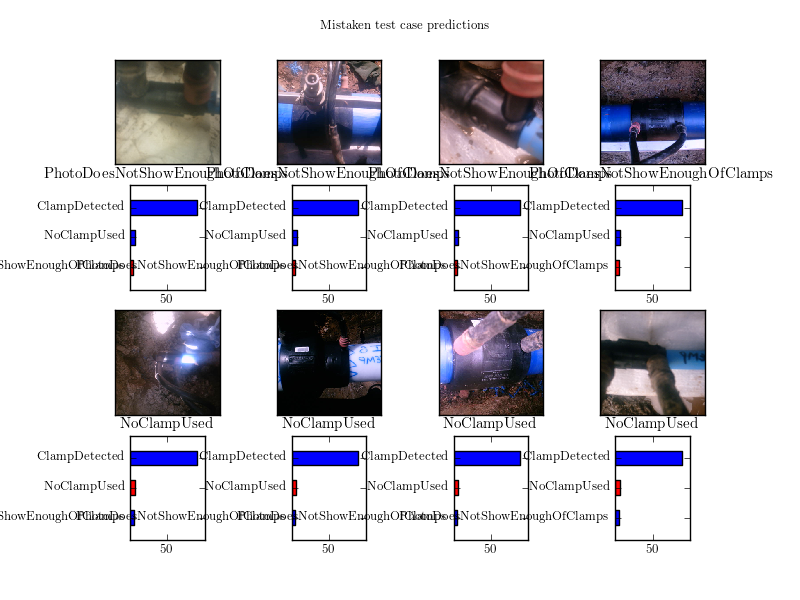
\includegraphics[scale=0.5]{images/preds9.png}
	\caption{test and validation error rates for clamp detection after setting momentum to zero}
\end{figure}

It can also be interesting to notice that no meaningful features are learned: for example, the filters learned at the lowest convolutional layer in optimised networks usually resemble edge or contrast detectors: in this case, they look noisy. 

\begin{figure}[h!]
	\centering
	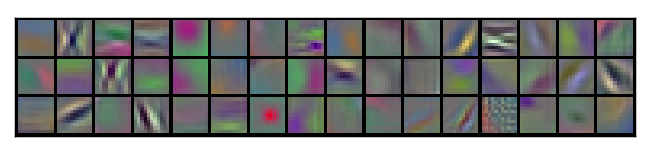
\includegraphics[scale=0.5]{images/good_filters.png} % need to crop to get side by side
	\caption{filters learned from a successfully optimised lowest convolutional layer} 
	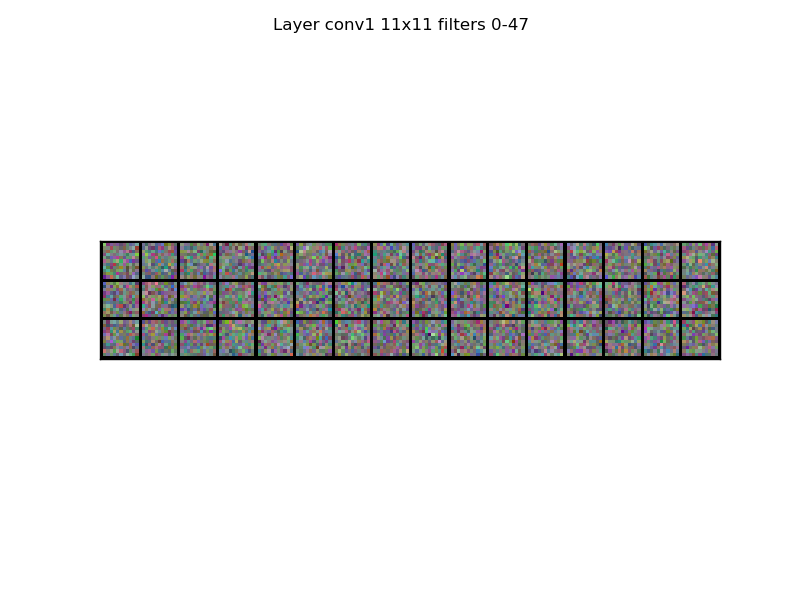
\includegraphics[scale=0.5]{images/bad_filters.png}  % need to crop to get side by side
	\caption{filters learned at lowest convolutional layer of this network}
\end{figure}

\subsubsection{Class Imbalance}

SHOULD I REALLY IMPLEMENT THIS? So much work just on the first task which was supposed to be preliminary... yes but you might as well do it now, you haven't got much else to do, since ControlPoint need to get round to sending me the extra metadata. Moreover, to get their confidence, you need to deliver good results. Transfer Learning is what I'm talking about boy. \\

Three approaches were taken to tackle class imbalance, the first ones being simplest to implement, the last ones most sophisticated and information-preserving. \\

\paragraph{Subset of Training Set}

CNNs were trained on all of the "No Clamps" or "Clamps Not Sufficiently Visible" images, and a random sample containing 15\% of the "Clamps Detected" images, in order to obtain an acceptably balanced dataset. This fix was easiest to implement and served as a benchmark for the more sophisticated subsequent approaches. Naturally, one would also expect this approach to be least effective: 85\% of the training data was lost, data which could intuitively serve not to teach the network to distinguish classes, but to learn features that are good encoders of pipe weld images, from which an effective discriminative setup of the parameters could ensue. \\

Note that the two minority classes were merged: because it is suspected that there is barely any semantic difference between them (will have to draw random samples to verify this), and because this reduces the number of majority class instances to remove, since it makes it easier to reach a good balance ratio. \\

Moreover, Bluebox images were chosen this time round, in order to limit the impact of mis-labelling and photographically poor images on training, and to limit the number of possible explanations for poor performance if that were to occur. According to ControlPoint the mis-labelling rate greatly decreased through time; since Bluebox images are the most recent, one would hope the mis-labelling rate would be lowest. However, this heavily reduced the amount of training data, requiring transfer learning to come into play. Still, just as a benchmark -- for the record -- randomly initialised AlexNets were trained from the ground up. \\

Since there is a tradeoff between class balance and dataset size, two different balance ratios were tested: 40\%/60\% for a dataset of and 33\%/66\%. \\ 

\paragraph{Partial Data Augmentation}

\paragraph{F Measure}


\clearpage
\section{Task 2: Transfer Learning}

\subsection{Motivations}

Because training set restricted. The objective here is to optimise transfer learning.
2 aspects: re-initialise weights, freeze backprop.

\subsection{Design}

\subsection{Implementation}

\subsubsection{Caffe}

Caffe is a framework for convolutional neural network algorithms, created by Yangqing Jia, and is in active development by the Berkeley Vision and Learning Center. It was chosen in order to implement transfer learning, or pretraining. Not like standard unsupervised pretraining, since this time, training was supervised, but on another dataset. So end result is pretty much the same, though it would be interesting to compare the two approaches. (unsupervised pretraining on ImageNet vs supervised pretraining on ImageNet). \\
 
The network pretrained on ImageNet is licensed for academic research, and is for non-commercial use only. Therefore, if ControlPoint wishes to make commercial use of a network whose weights were initialised from it, it would have to pretrain its own net on a dataset on which there are no such licensing restrictions. \\


\textit{Caffe Reference ImageNet Model: Our reference implementation of an ImageNet model trained on ILSVRC-2012 is the iteration 310,000 snapshot. The best validation performance during training was iteration 313,000 with validation accuracy 57.412\% and loss 1.82328. This model obtains a top-1 accuracy 57.4\% and a top-5 accuracy 80.4\% on the validation set.} \cite{caffe-website} \\

Contributed to Caffe by making it more space efficient: instead of the data being copied to the task directory, it is symlinked. The batching code tests for whether files are symlinks, and follows the link if that is the case. Caffe has a low-level tier written in C++ and a high-level tier written in Python; in this case, the modification was in C++. Note that before, it could get really inefficient to make copies of the data for every task. (One could use the same directory for several tasks, but if we want to keep control of class imbalance, we need flexibility in taking subsets of the training set. Therefore, one usually ends up requiring multiple different data directories, which makes the case for symlinked data all the more compelling.) \\

Caffe benchmark: https://github.com/soumith/convnet-benchmarks 

finetune_net.cpp calls solver.net()->CopyTrainedLayersFrom() then solver.Solve().

Does finetune chop off the top layer, or the top 2 layers? (Because DeCAF_6 better than DeCAF_7)
The answer to this should lie in CopyTrainedLayersFrom(param), in src/caffe/net.cpp
logs of which layers are copied are being sent to DLOG(INFO), seems that my output file does not receive it.
where can I get hold of DLOG? nevermind, just change it to send to LOG(INFO).
result: the following layers are copied: data conv1 relu1 norm1 pool1 conv2 relu2 norm2 pool2 conv3 relu3 conv4 relu4 conv5 relu5 pool5 fc6 relu6 drop6 fc7 relu7 drop7. fc8 is the only non-copied.

Does finetune do backprop on the top layer, or more?
1) The answer to this should lie in solver.Solve() in src/caffe/solver.cpp.

2) Another answer might be in Init() in net.cpp because it outputs "needs / does not need backward computation".
what matters is the point in the code at which "needs backward computation" is output, and from there work yourself up to which prototxt sets this.
looks like blobs_lr is the determinant param.  


Use L2 SVM linear support vector machine layer instead of softmax for transfer learning: http://arxiv.org/pdf/1306.0239.pdf
is it implemented in caffe?
https://github.com/BVLC/caffe/pull/398
https://github.com/BVLC/caffe/pull/303

proper transfer learning is extract features then train SVM:
http://arxiv.org/abs/1403.6382

this doesn't work as well with caffe:
https://github.com/BVLC/caffe/issues/642
works better with overfeat: http://cilvr.nyu.edu/doku.php?id=software:overfeat:start

if nevertheless you want to extract features with caffe:
http://caffe.berkeleyvision.org/gathered/examples/feature_extraction.html

or maybe with pylearn2: 
https://groups.google.com/forum/#!topic/pylearn-dev/hifIB5U-Gb8




\paragraph{leveldb}

More efficient implementation that does not require to create batches. Describe a bit what is going on under the hood, it seems that lookup tables are created for each image so that they can be dynamically pulled in (in constant time) to create batches on the fly. But find out more, it's cool. \\

\paragraph{Class Imbalance Solver}

Note that class imbalance ratio i.e.\ size of largest class relative to smallest class is not the right metric to consider. The right metric to consider is the proportion of the largest class, since this is what provides a bad/fake local minimum. This may not seem to be significant but it can be. Consider the 3 class case where we have 10, 100, 500 images for each respective class. Class imbalance ratio is 0.05, and proportion of largest class is approximately 0.82. If we wanted to attain a class imbalance ratio of 0.2, no class would be permitted to have more than 5*10=50 images, and we would be left with a training set of size 110. On the other hand, if we wanted to attain a proportion of largest class of 0.8, we would merely have to remove 12 images from the largest class, and we would be left with a training set of size 598. Interestingly, in the two class case, optimising with respect to either of the two metrics is equivalent. \\

Ok, but do we care about this for this project? Are we ever going to be training multi-class classifiers? Yes, if we think that it may help training to distinguish multiple cases. Intuitively, if two classes contain similar semantic content (e.g. inadequate clamp fitting and no clamp detected both involve clamps), then it could be better to train a single classifier on a 3-class task rather than 2 binary classifiers, because in the latter case, we lose potentially useful information that the images contain about clamps. In other words, to detect whether clamps are fitted properly, it helps to know what a clamp looks like, i.e.\ it helps to know which images do and don't have clamps. \\

t: target bad min
N: total number of current images
n: number of majority class images
k: number of majority class images to kill

when n-k is optimal, we have t = (n-k)/(N-k)
<=> t*N - t*k = n - k
<=> (1-t)*k = n - t*N
<=> k = (n-t*N)/(1-t) \\

so solution is to randomly delete n - n^* images from the majority class. \\

\subsubsection{Summary}

\subsection{Experimentation}

\subsubsection{Test Run}

Simple and Safe: very small, fixed learning rate throughout. Used all data, so high imbalance. Let's see whether class imbalance is as dangerous when only training the higher layers. \\

Significant improvement: 93.8\% validation error. The test error is: ??.\\

 


\subsubsection{Decreasing Learning Rate}

\paragraph{Step}

Caffe code:
 Return the current learning rate. The currently implemented learning rate
 policies are as follows:
    - step: return base $lr * gamma ^ (floor(iter / step))$
    
from src/caffe/solver.cpp:
if (lr_policy == "step") {
    int current_step = this->iter_ / this->param_.stepsize();

from src/caffe/proto/caffe.proto:
  optional int32 stepsize = 13; // the stepsize for learning rate policy "step"

These are all heuristics. No 2nd order methods involved. The intuition is that... Theory suggests that... . \\

Improvement: 94.5\% validation error. The test error is: ??.\\

\paragraph{Exp}

[...] \\

\subsubsection{Initialising Free Layers}

Use clampdet (threshold_freeze5/logs/1{3,4}-08-2014 to illustrate impact of initialising free layers to AlexNet weights or to randomly (re-)initialise them. Backprop enabled fully on all fc layers. \\

Both nets have frozen AlexNet conv[1-5] layers.
13 has 3 free fc layers with re-initialised weights
14 has 3 free fc layers transferred from AlexNet

So we expect 13 to do better.

Results: very convincing. 


\paragraph{Clampdet optimisation}

Wait a second. I got a bunch of clampdet detections high up in the 80s, but lately it's gone way down. Is small learning rate ruining it? 
"backprop on fc8, fc7 and biases of fc6" - start with alexnet weights - got 90\% - i.e.\ freeze5.5/
"backprop on fc8, fc7, fc6"              - start with alexnet weights - got 40\% - i.e.\ freeze5/14  

what the fuck!

5.5/11 has free fc[7-8],         semifree fc6 - step 10^-4 - 10^-4   - 85\%
5.5/12 has free fc[7-8],         semifree fc6 - inv  10^-5 - 10^-5   - 84\%
5.5/13 has free fc[7-8] new fc7, semifree fc6 - exp  10^-4 - 10^-6   - 40\%

11 and 12 are identical in train.prototxt.
But 13 is different in that fc7 is new!

Can the gap in performance be explained by lr_policy? or class imbalance opened up by re-initialisation?

To test this: 
14 is 13 with 11's lr_policy
15 is 11 with 13's lr_policy



\subsubsection{Freezing Backprop on various layers}

This section is a fucking mess. To bring order, you might have to train nets again. Structure should be as follows:
- pick a task: clampdet (easy) or hatch markings (hard)
- freeze backprop 1/2/3/4/5/6/7 layers
- import weights or re-initialise them
- learn on top of conv feature space of fc feature space

This would require training 2*7*2*2 = 56 nets. Not practical. Instead, when exploring either hyperparam, set the others to what you think is optimal. Also, if freeze 5 is less good than freeze k>5, no need to go lower. \\

\paragraph{Freeze Backprop on how many layers}

Fully enable 

Use clampdet (thresh, threshold_freeze{5.5,6,7}/logs/11-08-2014) to illustrate how the extent to which backrpop is freed up alters the expressive power of the network and its tendency to overfit (have you got a section in your paper explaining overfit? use the polynomials from Bishop, or the MLNC slides from A. Faisal to illustrate it, then link up with ). \\

Show that there is an optimal middle ground (i.e.\ non-monotonous error) number of layers to free up. In our case, freeing up top two layers is optimal. This middle ground is surprising: I'm surprised, I would expect more overfit when more layers are freed for backprop. Could anyone explain this?//

Soumith's opinion: Are you resetting the weights in the layers FC6,FC7 or are you just backproping from the AlexNet weights? I think if you reset the weights, you will see what you are expecting.\\
Me: Yeah, weights initialised to alexnet's. Why do you think that makes a difference? The local minima from alexnet's region leave less room for the net to learn meaningful patterns and push it more quickly into overfitting? \\ 
Soumith: when doing transfer learning, if you kept alexnet weights you are already in a well-settled local minima for that layer, so there wont be much movement I think.\\

The middle ground is possibly the result of a tradeoff: movement in function space versus over-expressiveness of the model. \\

\paragraph{Case 2: too much freeing}

Use scrape_zones/logs/1{3,4,5}-08-2014 to show that, with backprop freed up on all layers, even with transfer learning, expressiveness of model is such that (overfit or) bad_min occurs very quickly. 

13 is with all layers free. 14 is with fc8_new and fc7_new. 15 is with fc8_new only, and batchsize 512. Cannot constrain network more than 15, so if it fails, we're pretty screwed, that task is a really hard one. Might need an image transformation for scrape zones to stand out. In that case, delete or move this paragraph elsewhere more appropriate. \\


\paragraph{Case 3: hatch markings, combine both}

This section is a total mess, get rid of it, but stick descriptions in other hatch markings. \\

Freeing up too many layers leads to overfit, but preventing too many reduces expressive power of the net (show plots for {03,13}-08-2014). 13 freezes backprop up to weights of conv6, and re-initialises fc7 and fc8. \\

However 'CNN features of the shelf' figure 2a shows that training a linear SVM on the highest fc layer is best. So why not chop off the softmax layer for the 1000 imagenet classes, and add two layers? that way, images are projected onto the feature space given by the entire AlexNet, and a more expressive classifier than 1 single layer can be trained on it. This will also enable a more gradual funneling from the 4096 units of fc7 to the 2 unit softmax layer for the binary classification task. 512 and 2 unit fc layers are added onto top 7 layers of AlexNet. \\

Representing a SVM in a MLP: chaque neuron in bottom layer represente un datapoint. chaque neurone in layer above est associe a un support datapoint xi (support vector) et sa fonction d'activation est x -> K(xi,x). et tu as un neurone binaire dans la couche de sortie. \\

What's the difference between SVM and softmax in output? Learning minimizes a margin-based loss (maximise euclidean distance between nearest points and boundary) instead of joint probability of the data (i.e.\ the cross-entropy loss) {cite arxiv.org/pdf/1306.0239.pdf}. \\

Result: 14-08-2014, far worse than 13. So the real problem is all about lack of expressive power to bring training error to 0. \\

Note these results are surprising in light of 'CNN filters off the shelf', because closest there is to mimicking that paper here is 14. But you should properly benchmark 'CNN features off the shelf': use a linear SVM, so there is no kernel, just fitting hyperplanes. \\


\paragraph{Case 3: hatch markings, build on entire network or on conv layers only?}

Is there any use for the semantic information encoded in the fc layers? If the expressive power of the net is lost by freezing backprop on some fully connected layers, it seems we really need 3 fully free fully connected layers to make the most of the data.  \\

So: should these 3 fully free fc layers be put on top of AlexNet, or only the conv layers? In light of "intriguing properties" paper, a feature is not encoded in each fc neuron. So maybe there is no need to transfer its knowledge. \\

15-08-2014 has 3 fc new layers on top frozen conv[1-5] from AlexNet 
16-08-2014 has 3 fc new (random intialised) layers on top of frozen AlexNet (minus its softmax layer).

Note: batchsize bumped up to 256 for them both.

Results: 15 is significantly better, so information in fc layers is not as useful as raw filter information. In either case, model not expressive enough. \\


\paragraph{hatch markings optimisation}

We can summarise experimentation on hatch markings (so far) as:

03         has fully flexible AlexNet, all weights initialised to AlexNet
13         has 2 fc new layers on top frozen conv[1-5] and semifrozen fc_6 from AlexNet
14         has a funnel fc structure with 9 total layers, backprop on 2 new layers only
15-08-2014 has 3 fc new layers on top frozen conv[1-5] from AlexNet 
16-08-2014 has 3 fc new (random intialised) layers on top of frozen AlexNet (minus its softmax layer).

The conclusion is that a lot of expressive power is needed for this transfer task, and that the conv feature space is better than the fc feature space. \\

The worst is 14, because it has the least expressive power and starts 
but is has as much expressive power as 15, so it suggests filter feature space is better.
The best is 03, which suggests most important factor here is expressive power. 

More can still be done: 1) re initialise fc layers and 2) freeze backprop on lowest conv layers. Justification:
03 suffers from inheriting AlexNet fc weights. Perhaps backprop should also be frozen on its lowest conv layer(s) to prevent overfitting and because there's just no way those low level filters aren't optimal for this task too. 
Maybe re-initialising high level conv filters would help as well? Re-intialisation of only some kernel maps?

Next steps: best will be between 03 and 15: 3 fc new layers on top of conv layers, some of which are free, potentially even re-initialised. \\


\paragraph{hatch markings, optimisation II}

All nets now have 3 free fc new layers on top of 5 conv layers. Only conv layers remain to be optimised.
prototxt's edited from 15.

17 has fully flexible conv[2-5] layers (so like 03, but re initialise fc)
18 has fully flexible conv[4-5] layer

Results: both doing well. 5000 iterations not enough, keep going. SETUP TO RESUME

if 17,18 best so far, only fully flex conv[3-5] can be best
if 03,17 best so far, only fully flex conv[1-5] can be best
if 18,15 best so far, only fully flex conv5     can be best

Once you've settled that, another obscure possibility: re-initialise (part of) a conv layer. This might be likely if best so far has low conv layers: undoubtedly optimal low level features are getting sacrificed for the sake of model expressiveness. \\    


\subsubsection{Benchmark: 'CNN filters off the shelf'}

Implement OverFeat fc projection + linear SVM, and compare to your personal best. \\

To perform this benchmark correctly, need to use OverFeat and train a linear SVM. Your experiments with freezing backprop on caffe are similar but not identical, especially in light of that comment about caffe being weaker than OverFeat. \\

\clearpage
\section{Task 3: Class Imbalance}

\subsection{Motivations}

\subsection{Design}

\subsubsection{Threshold}

Papers: 
http://sci2s.ugr.es/keel/pdf/algorithm/articulo/2006%20-%20IEEE_TKDE%20-%20Zhou_Liu.pdf
http://www.eiti.uottawa.ca/~nat/Workshop2003/maloof-icml03-wids.pdf

It also allows you to assign different costs to the different misclassifications (i.e. if the algorithm is only supposed to flag potential problems then a false negative is much more expensive than a false positive)
the idea is that, if we have 2 classes and assign equal cost to both misclassifications, then we would want to pick the label with the biggest p(data | label) probability
however, the NN will compute the probabilities p(label | data) ~ p(data | label) p(label)
and a class imbalance means the priors p(label) are different
so you just need to correct for that by multiplying, for instance, the probability of p(label = 1 | data) outputted by the NN by the factor p(label=2) / p(label=1) and renormalizing \\

I get why it's called threshold: suppose p(c_1)=0.1. the threshold for classifying as c_1 moves from 0.5 to 0.1. Illustrate this point with one or two simple examples ("intuitively, ").  (that's pretty much what the "sig level" script I mentioned intends to do, except script has a flexible sig level.)
Also, I think that if we wanted to implement the threshold directly in the net, we might need to put the threshold layer after the softmax layer (and have it renormalise by 1/num_classes). cos it's non-linear so you can't be sure that their output will be renormalised in the same way. \\

Rather than have a fixed threshold hard-coded into the network, I propose to use a sig level script, for greater flexibility. \\


\subsubsection{Bayesian Cross Entropy Cost Function}

I also wonder whether it should be used in conjunction with a modified cost function. the threshold renormalisation won't change the fact that most of the error will come from c_2 examples, so the net would still be encouraged to learn c_2 more than c_1. [Provide a simple mathematical example of this]. If we want the stochastic gradient to reflect as much of the c_1 errors as the c_2 errors on average, then we need to renormalise the errors based on priors as well. This is done with bayesian cross entropy: [formula here] \\

When viewed as MLE estimation, the Bayesian cross entropy can be interpreted as follows: instead of trying to maximise the joint probability of the data under the assumption that each observed event has the same probability, we are assigning higher probability to minority class events. \\

\subsection{Implementation}

c++ threshold layer. bayesian softmax loss layer. bayesian layer abstract class with OOP from which the previous two inherit, which has access to minibatch labels and can compute the prior for the specific batch. More precise than assuming each minibatch has the same prior as the entire training set. \\

python script. \\



\subsubsection{Summary}


\subsubsection{Hardware}

CUDA-enabled GPU. How many teraflops? Which operations are parallelised? 
Moving from the GTX 780 to a Titan Black with ... \\

\subsection{Experimentation}

\paragraph{Is transfer learning more tolerant of class imbalance?}

Claim: there is more tolerance to class imbalance. Double check by looking at the error on a batch of minority class instances only.

Analytically: initialisation far from fake minima

Intuition for that is with initialisation, weights are in an area of the error surface that is far away from fake minima; the nearest local minima are more likely to be 'true' ones. Find evidence for this by viewing the features learned, and see whether they correspond to actual visual features. \\


\subsubsection{Soil Risk Contamination Task}

\paragraph{Test Run}

Class imbalance is very sharp, with only 3.9\% of soil contamination in the Bluebox images. So even with good initialisations from transfer learning, quite likely that network will not learn anything.

One should keep in mind that there could be a lot fake minima corresponding to "output majority class every time". The parameter space and the function space associated with every single parameterisation of a given deep neural network is not isomorphic; i.e.\ for a function, there exists many different parameterisations that can represent it. (Need to find a paper that goes into more depth on this.) \\

So even if backprop is frozen on all the lower layers to ensure that they are good feature detectors, it is still possible with just the use of the higher layers to generate a classifier that is nonsense from the point of view of learning representations of the classes at hand. As a result, fake minima can exist in the sweet spot region (sweet spot region as described by Yann LeCun's research). Since class imbalance is so sharp in this case, these fake minima are even deeper (they correspond to 96.1\% success rate), so they are likely to be deeper - and therefore accessible via gradient descent - than the true minima close to the point on the surface at which the network 'lands' with transfer learning. \\

\subparagraph{Training Results}

Validation error 0, at initialised weights:
Classification \% success: 0.125977
Cost function score: 1.35429

Validation error 1, after 50 mini-batch passes:
Classification \% success: 0.964844
Cost function score: 0.179662

Training error 0, at initialised weights:
Cost function score: 1.35429

Training error 1, after 1 mini-batch passes:
Cost function score: 0.179662

Training error 1, after 1 mini-batch passes:
Cost function score: 0.179662

(just have a plot of this! first 200 mini-batch passes). \\
Note no classification \% success because for efficiency reasons it is not computed by caffe for training batches.

\subparagraph{Observations}

Converges extremely quickly to 96\%. To confirm this, would have to run validation after every single minibatch pass. If that is indeed the case, then it tells us about how class imbalance litters the error surface with fake minima (one could emit the conjecture that the fake minima are as dense as the injectivity between parameter space and function space).

Stays in the 96\% region for the remaining mini-batch passes (have plot of all of those iterations). However the validation error is not always exactly the same - but if the validation is always using the exact same data and the net is indeed stuck at a fake minimum, shouldn't it always be the same value, i.e. the one corresponding to the exact proportion of majority class instances in the validation data? Check this!\\


\paragraph{Get more evidence}

Looking for evidence that in a given pot, there is a high number of fake minima all mapping to the same function that spits out majority class every time. If so, then the injectivity of parameter space into function space is not uniform: some functions can be represented by a lot more different parameterisations than others, and sadly for us, the bad function is one of the densely represented ones. Would be fantastic to come up with a toy example of this with a very simple network, but mathematically prove just how much more numerously certain functions can be represented than others. \\

One could empirically verify this by looking at what the network converges to with and without transfer learning. Also take very different initialisations for non transfer learning. If converged error rate same for all, and indeed sending in a batch of random images to each network spits out same or similar outputs every time, then we've got a few large scale examples as well. \\


\paragraph{Softmax Bayesian Loss Layer}

this concerns work done around 20th August. This was written on 23rd August. 

scrape_zones_sbl/22-08-2014: We look at the output probabilities, the loss values with and without bayesian renormalisation, the gradients for the softmax layer with and without bayesian renormalisation. 

We have a class imbalance of 81.5\%. In first train iteration, output probs are all close to (0.5, 0.5) i.e.\ with ~0.01 standard deviation. This makes intuitive sense, the network has no idea which class is more likely because it has learned nothing yet. \\

The SBL and SL losses are practically the same, they only vary by 0.15\%. This also makes sense: they will be different when the precision on one class differs markedly from the precision on the other class, which is not the case when outputting roughly (0.5,0.5) for every case. \\

The gradient backpropagated to the softmax layer is of dimension 2: one for each softmax neuron. It is interesting to note that grad(softmax_0) = - grad(softmax_1) always. So the modulus of the gradient for both softmax neurons is always the same, and the sign for softmax_i is given by whether softmax_i should have output a lower or a higher value. The reason for why the values are the same is because both neurons are always going to be the same distance away from the target value. This is only the case for 2 neurons. It might be interesting to think about how this property, which is only true for binary classifiers, affects training. \\

The SBL and SL gradients backpropagated to the softmax layer are instantly different: SBL gradient is always bigger than SL gradient for min class cases, and smaller for max class cases. Note, this is the case regardless of whether the prediction was correct or not. As a result, the weight updates 	

But wait: with SBL, do we really want to make the modulus bigger for both softmax neurons whenever we have a min class case? The answer would be yes, because we are going to update weights by the average gradient over the mini batch, so this is equalising the weight of the min class case (but it is adding noise to the gradient, because it's like replicating the same example - so it might lead to overfit actually). \\



So with SBL, do we really want to make the modulus bigger for both softmax neurons whenever we have a min class case? Or do we want to make the modulus bigger for the min class softmax neuron, for all class cases? Or both?
I think the latter corresponds to thresholding. So it is interesting to compare them. \\



\subsubsection{Tight Bowl Zig-zagging}

\subsubsection{Image Preprocessing}

Blurring if only colour matters, grey-scale if only shape matters, filter from ControlPoint. \\




\clearpage
\section{Conclusions and Future Work}

The realisation that weird sampling can heavily dent the approximation of the error surface has raised questions:

How does the training set provide an approximation of the true error surface? Since it can introduce dangerous minima, does that mean that, formally, it does not always provide an extrema-conserving approximation of the true error surface? Theoretically, what are the conditions for obtaining an extrema-conserving approximation (i.e. that doesn't introduce fake minima)? Practically, can we perform transformations on the cost function, or do stuff to our data (sampling), to limit the introduction of fake minima?  \\

Could we answer these questions if, instead of facing the usual problem of having a training set sampled from an unknown distribution, we ran a completely artificial experiment where we start with a known distribution? That way, we know the true error surface, and as we draw samples from the distribution, we can look at how each one approximates the true error surface, how it introduces bad minima? \\

How does mis-labelling alter the error surface? Intuitively, it would seem that it lifts up the true minima only, making the false minima even more attractive (e.g.\ "labelling is so bad it's too confusing, there's just nothing to distinguish them, so I might as well go for the blind strategy of outputting clamp detected all the time"). \\

because exists injection of parameter space into function space, and because of what Yann says, can view the error surface as a replication of side-by-side identical pots with jagged bottom. However, seeing as we run into imbalance-induced fake minima with transfer learning as well, despite
Conjecture that imbalance-induced fake minima are littered across the entire error surface, also present in the sweet spot zone. Conjecture further that they are as dense as the relative size between parameter space and function space. Could be interesting to think about how the choice of a network architecture affects this injectivity.

Unsupervised Learning to correct mis-labelling, with encouragements to create clusters initialised by those resulting from supervised learning (maybe could only work well with many false negatives, few false positives, as is the case here?). \\ 


\begin{thebibliography}{1}
% Example: \bibitem{One}
% a better way of doing it: a .bib file or something. bit.ly/1kqg2Qe
\bibitem{decaf}
 Donahue, Jeff; Jia, Yangqing; Vinyals, Oriol; Hoffman, Judy; Zhang, Ning; Tzeng, Eric; Darrell, Trevor;
  \emph{DeCAF: A Deep Convolutional Activation Feature for Generic Visual Recognition}\\
  arXiv preprint arXiv:1310.1531, 2013

\bibitem{MIML}
 Zhou, Zhi-Hua; Zhang, Min-Ling;
  \emph{Multi-Instance Multi-Label Learning with Application to Scene Classification}\\
  Advances in Neural Information Processing Systems 19, 
  Proceedings of the Twentieth Annual Conference on Neural Information Processing Systems, 
  Vancouver, British Columbia, Canada, 
  December 4-7, 2006

\bibitem{f-measure}
 Pastor-Pellicer, Joan; Zamora-Martinez, Francisco; Espana-Boquera, Salvador; Castro-Bleda, Maria Jose;
  \emph{F-Measure as the Error Function to Train Neural Networks}\\

\bibitem{control-point}
 Fusion Group - ControlPoint LLP,
 \emph{Company Description}\\
 URL: \url{http://www.fusionprovida.com/companies/control-point}, last accessed 5th June 2014. 
  
\bibitem{univ-approx}
 Barron, Andrew R.,
 \emph{Universal Approximation Bounds for Superpositions of a Sigmoidal Function}\\
 IEEE Transactions on Information Theory, 
 Vol. 39, No. 3
 May 1993

\bibitem{DL-book}
 Bengio, Yoshua;
 \emph{Learning Deep Architectures for AI}\\
 Foundations and Trends in Machine Learning, 
 Vol. 2, No. 1 (2009) 1-127
 2009

\bibitem{Russel & Norvig}
 Russell, Stuart J; Norvig, Peter;
 \emph{Artificial Intelligence: A Modern Approach}\\
 2003

\bibitem{krizhevsky}
 Krizhevsky, Alex; Sutskever, Ilya; Hinton, Geoffrey E.;
 \emph{ImageNet Classification with Deep Convolutional Neural Networks}\\
 2012

\bibitem{rectifier}
 Glorot, Xavier; Bordes, Antoine; Bengio, Yoshua;
 \emph{Deep Sparse Rectifier Neural Networks}\\
 2013

\bibitem{MLP-univ-approx}
 Hornik, Kur; Stinchcombe, Maxwell; White, Halber;
 \emph{Multilayer Feed-Forward Networks are Universal Approximators}\\
 1989

\bibitem{office}
 Saenko, K., Kulis, B., Fritz, M., and Darrell, T.;
 \emph{Adapting visual category models to new domains}\\
 ECCV, 2010

\bibitem{surf}
 Bay, H., Tuytelaars, T., and Gool, L. Van;
 \emph{SURF: Speeded up robust features}\\
 ECCV, 2006

\bibitem{transfer-learning}
 Sermanet, Pierre; Eigen, David; Zhang, Xiang; Mathieu, Michael; Fergus, Rob; LeCun, Yann;
 \emph{OverFeat: Integrated Recognition, Localization and Detection using Convolutional Networks}\\
 arXiv:1312.6229
  
\bibitem{f-measure}
 Joan Pastor-Pellicer, Francisco Zamora-Martínez, Salvador España-Boquera, María José Castro-Bleda;
 \emph{F-Measure as the Error Function to Train Neural Networks}\\
 Advances in Computational Intelligence
 Volume 7902, 2013, pp 376-384
 
\bibitem{cuda-convnet}  
 URL: \url{https://code.google.com/p/cuda-convnet/}, last accessed 6th June 2014.

\bibitem{caffe-website}  
 URL: \url{http://caffe.berkeleyvision.org/getting_pretrained_models.html}, last accessed 6th June 2014.

\bibitem{nips-tut}  
 URL: \url{http://research.microsoft.com/apps/video/default.aspx?id=206976&l=i}, last accessed 6th August 2014.


\end{thebibliography}

\end{document}
